\documentclass[fleqn,twoside]{article}
\usepackage[utf8]{inputenc}

%margins and size of page
\usepackage[twoside, top=3.0cm,bottom=3.0cm,right=2.5cm,left=2.5cm]{geometry}
\setlength{\oddsidemargin}{0mm} 
\setlength{\evensidemargin}{0mm} 

%1.5 line spacing
\renewcommand{\baselinestretch}{1.5} 

%for changing text sizes
\usepackage{mathptmx}
\usepackage{anyfontsize}
\usepackage{t1enc}

%changing space under headings
\usepackage{titlesec}

%figure placement
\usepackage{float}% If comment this, figure moves to Page 2

%table manipulation
\usepackage{supertabular,booktabs,tabularx}
\usepackage{ltablex}
\usepackage{booktabs}
\usepackage{rotating}
\usepackage{array}

\newcolumntype{C}{>{\centering\arraybackslash}X} % centered version of "X" type


%roman numerals
\usepackage{enumerate}% http://ctan.org/pkg/enumerate

%math tools
\usepackage[cmex10]{amsmath}
\usepackage[cmex10]{amsmath,mathtools}
\usepackage{fixltx2e}
\setlength{\mathindent}{0pt} %left align

%\titlespacing*{<command>}{<left>}{<before-sep>}{<after-sep>}
\titlespacing*{\section}    %main heading
{0pt}{5.5ex plus 1ex minus .2ex}{0ex plus .2ex}
\titlespacing*{\subsection}    %subheading
{0pt}{5.5ex plus 1ex minus .2ex}{0ex plus .2ex}
\titlespacing*{\subsubsection}    %subsubheading
{0pt}{5.5ex plus 1ex minus .2ex}{0ex plus .2ex}

%subsubsubsection 
\setcounter{tocdepth}{4}
\setcounter{secnumdepth}{4}

%nomenclature
\usepackage{nomencl}
\makenomenclature

%images
\usepackage{graphicx}
\graphicspath{ {images/} }
\usepackage{pdfpages}


%symbols
\usepackage{amssymb}


%for subfigures - side by side figures
\usepackage{caption}
\usepackage{subcaption}

%wrapped figures
\usepackage{wrapfig}

%header info
%\usepackage{fancyhdr}
%\pagestyle{fancy}
%\fancyhead[LO,LE]{} %remove automatic left headers
%\rhead{6007ENG - Industry Affiliate Program, Semester 1, 2015}

%footer line
%\renewcommand{\footrulewidth}{0.4pt}% default is 0pt

%paragraph - no indent with space
\usepackage[parfill]{parskip}

%bibliography
%\usepackage{biblatex}
\usepackage[square, numbers, comma, sort&compress]{natbib}

%appendix
\usepackage[toc,page]{appendix}


% *** PDF, URL AND HYPERLINK PACKAGES ***
%
\usepackage{url}
\usepackage{hyperref}
% url.sty was written by Donald Arseneau. It provides better support for
% handling and breaking URLs. url.sty is already installed on most LaTeX
% systems. The latest version and documentation can be obtained at:
% http://www.ctan.org/tex-archive/macros/latex/contrib/url/
% Basically, \url{my_url_here}.



% correct bad hyphenation here
\hyphenation{op-tical net-works semi-conduc-tor}



%%%%%%%%%%%%%%%%%%%%%%%%%%%%%%%%%%%%%%%%%%%%%%%%%%%%%%%%%%%%%%%%%%%%%%%%%%%%%%

\begin{document}
%stop space between paragraphs
\raggedbottom

\begin{titlepage}

% Declare new goemetry for the title page only.
\newgeometry{top=4.0cm,bottom=1cm,right=2.5cm,left=2.5cm}
%---------------------------------------------

\newcommand{\HRule}{\rule{\linewidth}{0.5mm}} % Defines a new command for the horizontal lines, change thickness here
 
\begin{flushleft} 
 

%----------------------------------------------------------------------------------------
%	Title section
%----------------------------------------------------------------------------------------


{ \Huge \bfseries Machine vision approach to identifying and grading Strawberries}\\[1.5cm] % Title of your document

%----------------------------------------------------------------------------------------
%	Name section
%----------------------------------------------------------------------------------------

\textsc{\Large \bfseries Mr. Gilbert Eaton --- BIT/BEng (Hons. I)}\\[0.5cm] % course title
 
 
 
\vspace{10mm} 


%----------------------------------------------------------------------------------------
%	Supervisor information SECTION
%----------------------------------------------------------------------------------------

\textsc{\Large \bfseries Magnificent Pty. Ltd.}\\[0.5cm] % Name of school
\textsc{\Large \bfseries Griffith University}\\[0.5cm] % Name of uni
\textsc{\Large \bfseries School of Engineering - Griffith Sciences}\\[1.5cm] % course title

%----------------------------------------------------------------------------------------
%	Disclaimer SECTION
%----------------------------------------------------------------------------------------

\emph{A report submitted in partial fulfilment of the degree of Doctor of Philosiphy, and in confidence due to the agreement with ARC Linkage partners}\\[1.5cm]


%----------------------------------------------------------------------------------------


\end{flushleft}

\vfill % Fill the rest of the page with whitespace

\end{titlepage}

% Ends the declared geometry for the titlepage
\restoregeometry
%--------------------------

%adds roman numerals to the TOC
\pagenumbering{roman}

%%%%%%%%%%%%%%%%%%%%%%%%%%%%%%%%%%%%%%%%%%%%%%%%%%%%%%%%%%%%%%%%%%%%%%%%%%%%%%

%----------------------------------------------------------------------------------------
%	Abstract
%----------------------------------------------------------------------------------------


\section*{Abstract}

%adds unnumbered section to TOC
\addcontentsline{toc}{section}{ABSTRACT}



\vspace*{\fill}%


%%%%%%%%%%%%%%%%%%%%%%%%%%%%%%%%%%%%%%%%%%%%%%%%%%%%%%%%%%%%%%%%%%%%%%%%%%%%%%


%----------------------------------------------------------------------------------------
%	Statement
%----------------------------------------------------------------------------------------
\newpage

\section*{Statement of Originality}
\addcontentsline{toc}{section}{Statement of Originality}

This work has not previously been submitted for a degree or diploma in any university. To the
best of my knowledge and belief, the thesis contains no material previously published or writtenby another person except where due reference is made in the thesis itself.

\vspace{50pt}

signed
Gilbert Eaton

\vspace*{\fill}%

%%%%%%%%%%%%%%%%%%%%%%%%%%%%%%%%%%%%%%%%%%%%%%%%%%%%%%%%%%%%%%%%%%%%%%%%%%%%%%


%----------------------------------------------------------------------------------------
%	Acknowledgements
%----------------------------------------------------------------------------------------
\newpage

% use section* for acknowledgement
\section*{Acknowledgements}

%adds unnumbered section to TOC
\addcontentsline{toc}{section}{Acknowledgements}

The author would like to acknowledge Griffith University staff Rudi Bartels, Dr. Andrew Busch and Prof. Yongsheng Gao for their guidance and knowledgeable advise during the project. Thanks also go to William Sheng who has been working on the project and provided invaluable knowledge.

....

\vspace*{\fill}%

%%%%%%%%%%%%%%%%%%%%%%%%%%%%%%%%%%%%%%%%%%%%%%%%%%%%%%%%%%%%%%%%%%%%%%%%%%%%%%


%----------------------------------------------------------------------------------------
%	Publications
%----------------------------------------------------------------------------------------
\newpage

% use section* for acknowledgement
\section*{Publications}
%adds unnumbered section to TOC
\addcontentsline{toc}{section}{Publications}


\subsection{First-Author Publications}

\begin{itemize}
	\item{G. Eaton, A. Busch, R. Bartels, Y. Gao, “A Method To Create Stable Lighting And Remove Specular Reflections for Vision Systems”,Digital Image Computing: Techniques and Applications (DICTA), DOI: 10.1109/DICTA.2017.8227392 (2017)}
	\item{G. Eaton, A. Busch, R. Bartels, Y. Gao, “Colour Analysis of Strawberries on a Real Time Production Line”, Digital Image Computing: Techniques and Applications (DICTA), (2018)}
	\item{Coming soon......}
\end{itemize}  



\vspace*{\fill}%

%%%%%%%%%%%%%%%%%%%%%%%%%%%%%%%%%%%%%%%%%%%%%%%%%%%%%%%%%%%%%%%%%%%%%%%%%%%%%%

%----------------------------------------------------------------------------------------
%	table of contents/figs/tables/nomenclature
%----------------------------------------------------------------------------------------

%1.0 line spacing
\renewcommand{\baselinestretch}{1.0} 
%contents
\newpage
\tableofcontents

%figures
\newpage
\listoffigures

%tables
\newpage
\listoftables

%nomenclature
\newpage
%Strawberry jargon
\nomenclature{$cultivar$}{The species or type of fruit}%
\nomenclature{$punnet$}{A plastic strawberry container}%
\nomenclature{$calyx$}{The green leaves and stem attached to strawberry}%
\nomenclature{$downtime$}{The amount of time (cumulative) during production where nothing is produced}%
\nomenclature{$a$}{}%
\nomenclature{$b$}{}%


%cvip jargon
\nomenclature{$SVM$}{Support Vector Machine}%
\nomenclature{$RBF$}{Radial Basis Function}%
\nomenclature{$AI$}{Artificial Intelligence}%
\nomenclature{$BP$}{Back Propogation}%
\nomenclature{$FC$}{Fully Connected (NN layer)}%
\nomenclature{$ReLU$}{Rectified Linear Unit}%
\nomenclature{$NN$}{Neural Network}%
\nomenclature{$ANN$}{Artificial Neural Network}%
\nomenclature{$FNN$}{Feedforward Neural Network}%
\nomenclature{$CNN$}{Convolutional Neural Network}%
\nomenclature{$BPNN$}{Back-propogation Neural Network}%
\nomenclature{$k-NN$}{k-Nearest Neighbour}%
\nomenclature{$DNN$}{Deep Neural Network}%
\nomenclature{$ELM$}{Extreme Learning Machine}%
\nomenclature{$SFLN$}{Single Hiden Layer Feed Neural Network}%
\nomenclature{$MLP$}{Multi-layer Perceptron}%
\nomenclature{$GMM$}{Gaussian Mixture Model}%
\nomenclature{$PCA$}{Principal Component Analysis}%
\nomenclature{$IR$}{Infra-Red}%
\nomenclature{$RGB$}{Red, Green, Blue}%
\nomenclature{$HSI$}{Hue, Saturation, Intensity}%
\nomenclature{$HSV$}{Hue, Saturation, Value}%
\nomenclature{$CIELAB$}{CIE standard colourspace}%

%computer jargon
\nomenclature{$UI$}{User Interface}%
\nomenclature{$PC$}{Personal Computer}%
\nomenclature{$PSU$}{Power Supply Unit}%
\nomenclature{$UPS$}{Uninterruptable Power Supply}%
\nomenclature{$CPU$}{Central Processing Unit}%
\nomenclature{$GPU$}{Graphical Processing Unit}%
\nomenclature{$AVX$}{Advanced Vector Extensions}%

%photography jargon
\nomenclature{$FOV$}{Field of view}
\nomenclature{$LED$}{Light emitting diode (Light source)}
\nomenclature{$CCD$}{Charge coupled device (sensor)}
\nomenclature{$CMOS$}{Complimentary metal-oxide semiconductor (sensor)}

%mechanical
\nomenclature{$DOF$}{Degrees of Freedom}


%Sequence to make nomenclature refresh is:
%1 - Compile
%2 - Command - use terminal for the following:
%		C:\\>makeindex -s nomencl.ist -o Gilbert_Eaton_PHD.nls Gilbert_Eaton_PHD.nlo
%3 - Compile
\renewcommand{\baselinestretch}{0.5} 
\printnomenclature

%1.5 line spacing
\renewcommand{\baselinestretch}{1.5} 

%footer change
%\fancyfoot[CO, CE]{}
%\fancyfoot[RO] {\thepage}
%\fancyfoot[LO] {Gilbert Eaton}
%\fancyfoot[RE] {Quality Checking Strawberries using Multi-spectral Imaging}
%\fancyfoot[LE] {\thepage}

%%%%%%%%%%%%%%%%%%%%%%%%%%%%%%%%%%%%%%%%%%%%%%%%%%%%%%%%%%%%%%%%%%%%%%%%%%%%%%
%%%%%%%%%%%%%%%%%%%%%%%%%%%%%%%%%%%%%%%%%%%%%%%%%%%%%%%%%%%%%%%%%%%%%%%%%%%%%%

%changes back to numeric page numbering
\pagenumbering{arabic}
\newpage

\section{Introduction}

Machine vision systems have been successfully deployed to perform many tasks in industries such as manufacturing, automotive, mining, and is constantly branching into more diverse fields, for example, vehicle guidance \cite{menze,urmson}, drone applications \cite{greene,boucher}, traffic monitoring \cite{cheung,kamijo}, high-speed vision \cite{watanabe,nakabo}, and quality inspection tasks \cite{cubero, du}. This is due, largely, to recent technology advances in computational devices (CPU/GPU), storage and cloud services, and camera technology and affordability. These factors help in the adoption of machine vision for production quality control in order to provide multiple benefits over human inspection which may include labour cost reduction, consistent objective analysis, speed increases, safety risk reduction, and continuous services. Avoiding costly stock returns is an obvious benefit, however many costs can be unquantifiable or unclear such as customer satisfaction, brand reputation.

Production line quality inspection is one of the most common applications for machine vision as it is usually fixed in position with a known area to assess, giving the cameras opportunity to inspect each and every item produced. The cameras are also capable of working in environments that human operators may not tend to be comfortable in. Where the production lines may be exposed to heat, cold, dust, chemical, pressure, or noise hazards, cameras can solve the problem of human risk. 

Cameras can be used for high-speed moving objects in order to perform the inspections where a human would have an impossible task. For example Duan et al \cite{duan} used a system of two cameras and two computers to inspect glass beer bottles after production at a rate of $500/min$ or $8.3/s$. They inspected the bottom of the bottle, the overall finish, and the top opening, performign all three checks for each bottle within the timeframe specified. After inspection, the defected bottles are ejected from the production line in order to be recycled. Elmasry et al \cite{elmasry1} developed a potato grading system which can acquire multiple images of each potato, from multiple sides due to the roller-conveyor, before performing Fourier transform, and Fourier shape descriptors. The conveyor speed is $1m/s$ and the spacing between each roller is $80mm$ giving approximately $12 potatos/s$ if there are no empty rollers. Four different grading/processing techniques were investigated by Kondo \cite{kondo} where, firstly, oranges were inspected by a system of cameras including six colour cameras at different positions (so that all sides are inspected), an NIR camera and the option of adding x-ray imaging to the purpose-built line. The oranges are fed through the system using a singulating conveyor which performs a $180^{circ}$ rotation for the last camera to ensure all sides are evaluated. Secondly, an eggplant quality assemsment system was developed which made use of six colour and four monochrome cameras in order to determine colour, size, shape, and defects as well as a novel gloss detection method using angles cameras and three white strip lights to inspect the specular reflections sharp edges, meaning good quality, or dull edges, meaning poor. The 6 production lines, running at $38.1m/min$, at the facility meant that $504,000$ fruits could be processed per day. Even though there has been a substantial reduction in number of employees in processing, it is still laborious due to the packing requirements. The third project was capable of grading $10,000$ leeks per hour at a line speed of $30m/min$ with automatic root cutting and peeling steps. Lastly, a robot capable of grading $3 fruit/sec$ for 11 varieties of deciduous fruits including apple, pear, and peach. Using 3 DOF manupulators, the robot placed into trays, whilst images are acquired from top, bottom and two sides before making a grade decision. This shows that for fast moving production lines, humans are unable to peform the necessary tasks to quality inspect each item. The high speed vision systems are tailored to suit each application and are dependant on good lighting due to the rapid shutter speeds of the camera.




\begin{figure}[ht]
	\centering
	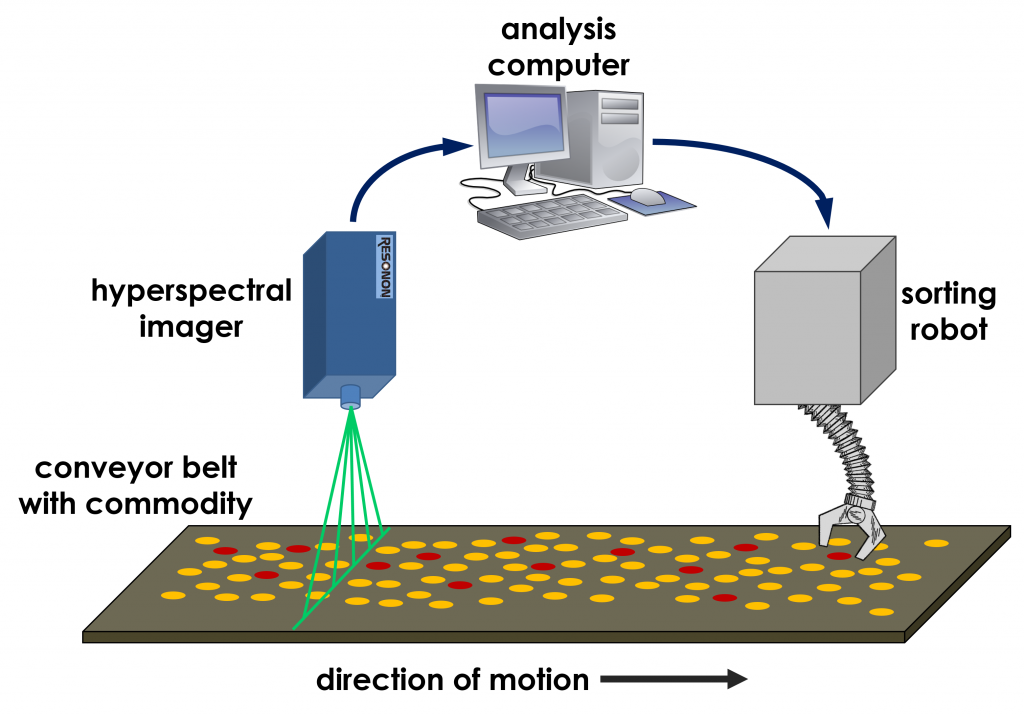
\includegraphics[width=300pt]{images/machine_vision.png}
	\caption{Example of production line using multi-spectral acquisition system with a robotic arm sorting the objects.}
	\label{fig:machine_vision}
\end{figure}

Most production line vision systems have a control mechanism that removes any defected items and allows only acceptable quality to pass. A basic diagram of this process is shown in Figure \ref{fig:machine_vision} whereby a camera provides information to the PC to decide which objects to accept and reject, while a mechanical device removes unacceptable items. 




\subsection{Industry Partner}

Magnificent Pty. Ltd. is a strawberry farming and processing company located in Wamuran, Queensland. In this facility (as well as the company's secondary strawberry farm in South Australia), the company plants, grows, maintains, picks, and packs the berries ready for consumer purchase. Ray Daniels has operated the 100$ha$ farm for over 20 years in Wamuran, and has recently acquired a new, smaller 26$ha$ farm in Myponga, SA. Magnificent employs around 250 people in the peak of the season and consists of planting, picking, packing, driving (tractors/trucks) and operator teams. Producing around 1.7 million $kg$ of strawberries each year, Magnificent has a good market share with many high-profile customers including major supermarket chains such as Coles, IGA, and CostCo. The company has it's own transportation and storage facilities allowing for a distribution centre in Brisbane, Queensland's capital city. 

The Strawberries are picked and packed by hand using labour intensive methods in order to produce the finished goods, which can be sold in many different sized packages from 250g through to 3kg jumbo pack. The strawberries are packaged according to the quality grade or cultivar, however, if the fruit is in high demand or weather conditions cause shortages in supply, the lower grades can be used as high grade berries making the classification depend on market conditions.

Due to environmental and market demands, the standard of strawberries packed can vary between seasons, and as Magnificent employs a mostly casual workforce, the standard can differ between days also. Each operator must pack the correct weight, into the correct container, as fast as possible, whilst ensuring that there are no defected berries from a range of attributes such as over/under ripe, bruising, foreign objects, pest damage, dirt and soil, size, shape and overall appearance. This evaluation can be difficult in this fast-paced environment and could be easily overlooked in situations under pressure, especially when concerned with bruising. Bruising can be hard to detect, even for the trained eye, as the colour and texture takes some time to decay to an unacceptable level. The time taken to decay could be several hours to a few days and, as there may be up to 5 days transport time for berries picked by Magnificent, this leads to the case where finished product has left the distribution centre quality assured, but is rejected when it arrives at the destination. Magnificent are regularly given feedback from their customers regarding the quality of each punnet after it reaches it's destination point anywhere throughout Australia. Whilst training and education regarding these quality specifications is given, this will be lost as soon as the workforce is replaced by a new season of employees.  


\begin{figure}[h]
	\centering
	\begin{subfigure}{.4\textwidth}
		\centering
		
\includegraphics[width=.6\linewidth]{sunray.jpg}
		\caption{}
		\label{fig:sunray}
	\end{subfigure}%
	\begin{subfigure}{.6\textwidth}
		\centering
		\includegraphics[width=.8\linewidth]{whatwedo_logo.jpg}
		\caption{}
		\label{fig:whatwedo}
	\end{subfigure}%
	\caption{(a) Magnificent logo, (b) Workers and fields at Magnificent}
	\label{fig:test}
\end{figure}

In order to reduce costs and improve efficiencies, Magnificent has invested in various projects to bring a technological approach to farming. Some of these include a strawberry harvesting robot which must navigate through the fields many rows of planting mounds, picking strawberries \cite{busch}. A greenhouse picking system was also developed, where specialised planting troughs were constructed to bring the strawberries to the harvester using a vertical farming method. The company has also connected it's information systems together using a variety of applications interfaced to hardware such as weigh scales and employee clock-in stations. This gives better visibility to the managers and operators to make decisions in a real-time environment. 




\subsection{Project Description and Requirements}


Since 2015, the strawberry packing line has been fitted with a machine that seals the lids on the punnets with plastic film instead of using a resealable lid. This measure has been adopted for a few reasons, namely, cost of packaging, ease of packing, and anti-tampering properties. Shown in Figure \ref{fig:heat_seal}, the heat-seal machine has a maximum speed of $120 punnets/min$ or $2 punnets/s$ and seals six punnets per cycle which improves the overall efficiency. Given that the machine must press down onto the stationary punnets with the heating elements, increasing the amount that can be sealed at once, increases throughput rate. However, the length of the heat-seal footprint is correlated to the number of punnets sealed per cycle. As there is limited space, the amount which can be processed simultaneously is also limited. The infeed conveyors must account for this batching of punnets by stopping when the sealing compartment is loaded, and starting when unloaded. The stop-start action is surpressed by an accumulator conveyor running at a slower speed and gradually feeding into the baching section, but still requires the infeed to stop, albeit a lesser frequency. This means when integrating production conveyors to feed this machine, the discontinuous nature of the flow of punnets must be considered.


\begin{figure}[ht!]
	\centering
	\begin{subfigure}{\textwidth}
		\centering
		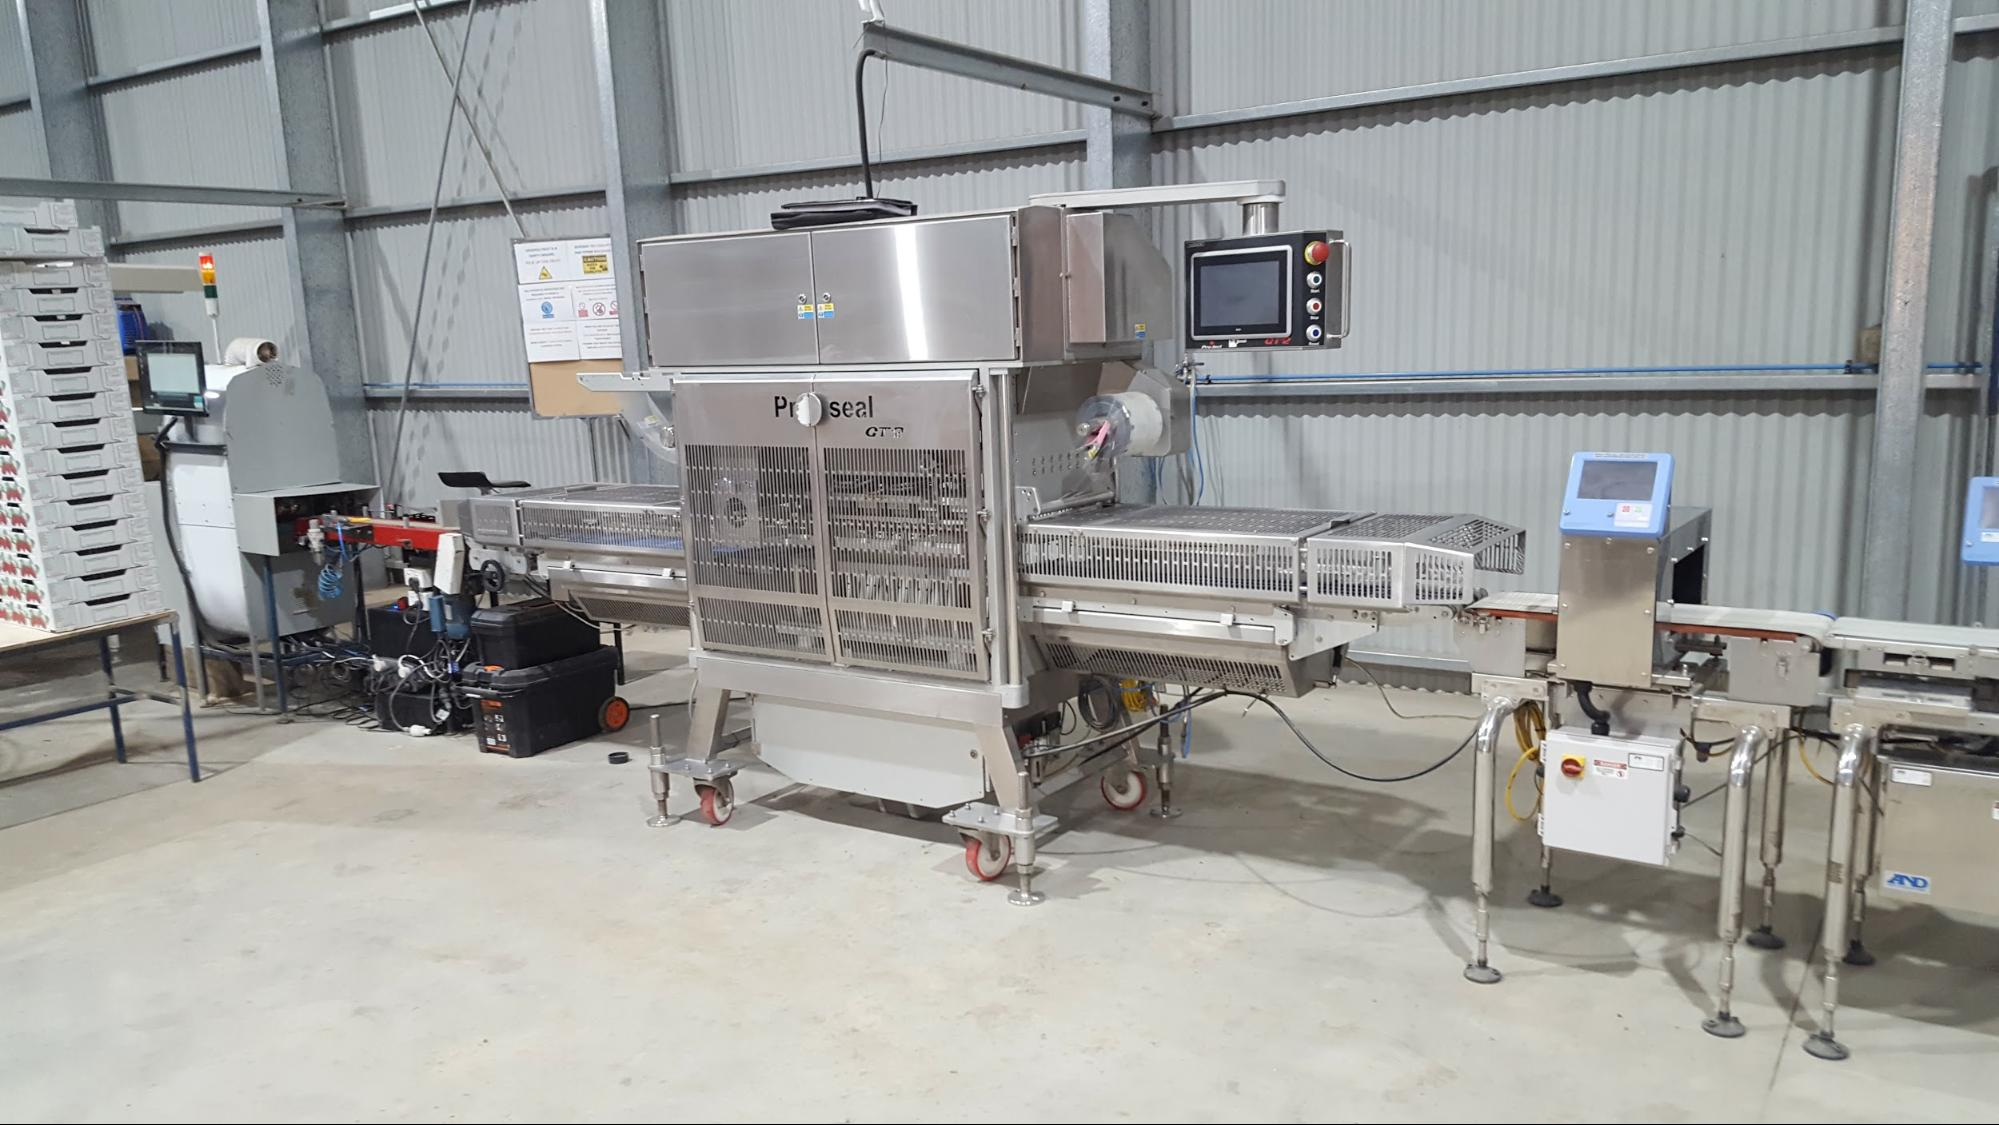
\includegraphics[width=.8\linewidth]{heat_seal.jpg}
		\caption{}
		\label{fig:heat_seal}
	\end{subfigure}%
	
	\begin{subfigure}{.5\textwidth}
		\centering
		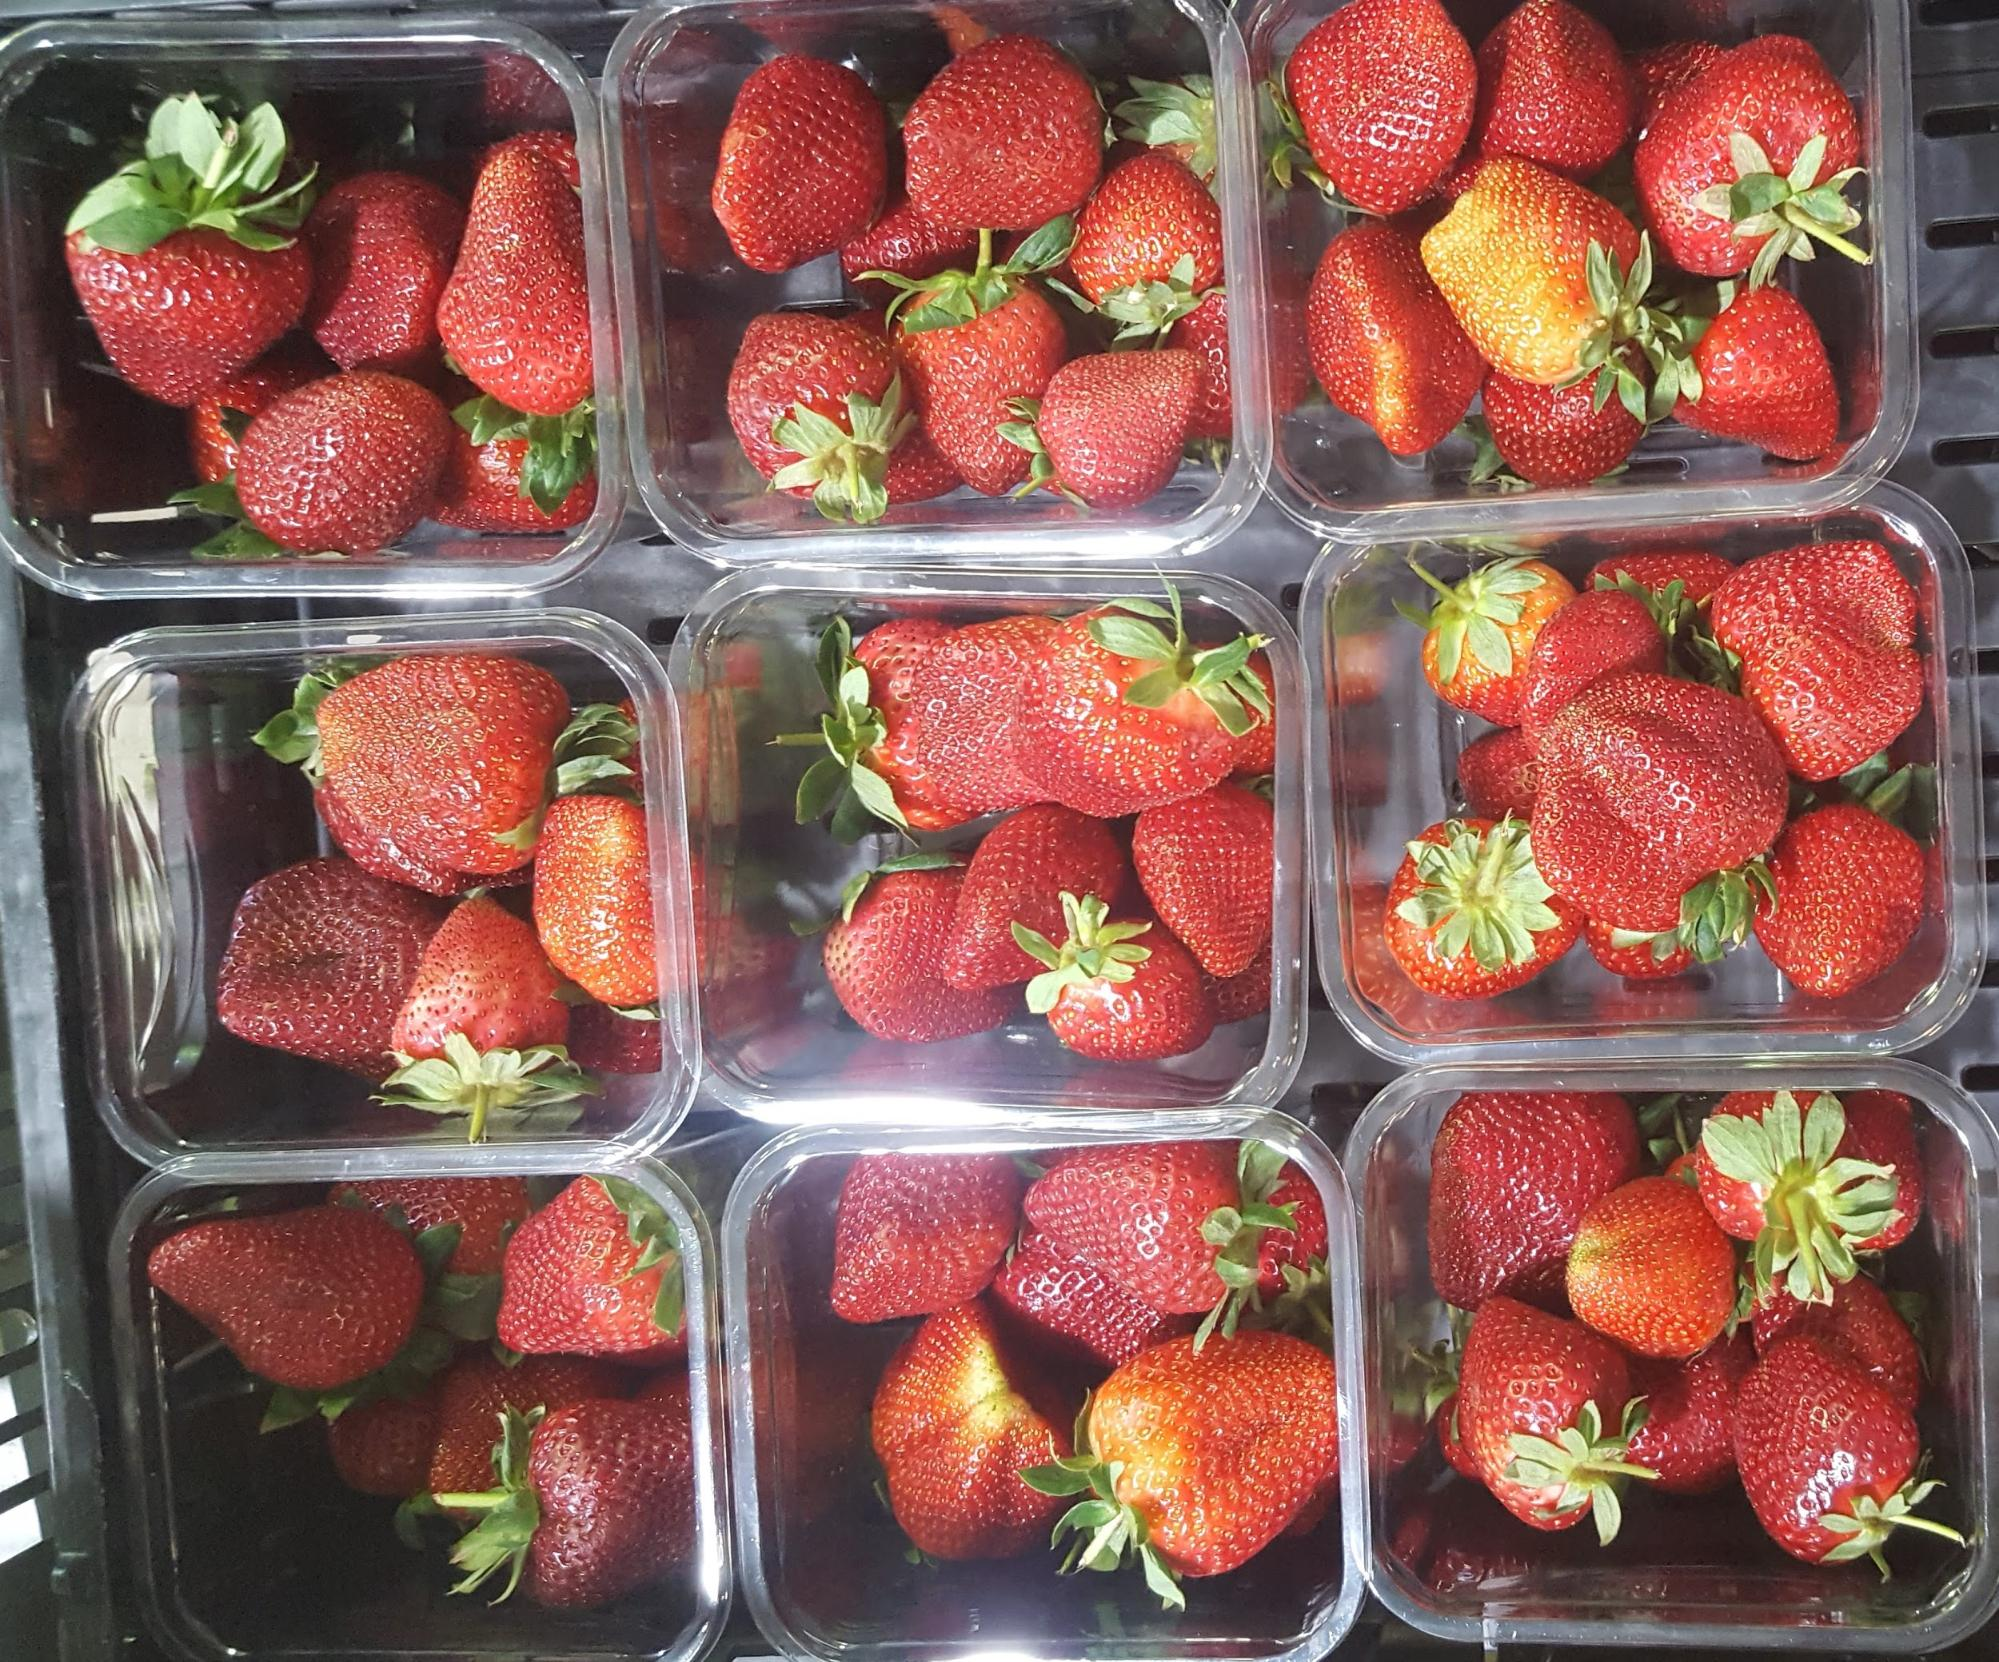
\includegraphics[width=.6\linewidth]{unsealed_punnets.jpg}
		\caption{}
		\label{fig:unsealed_punnets}
	\end{subfigure}%
	\begin{subfigure}{.5\textwidth}
		\centering
		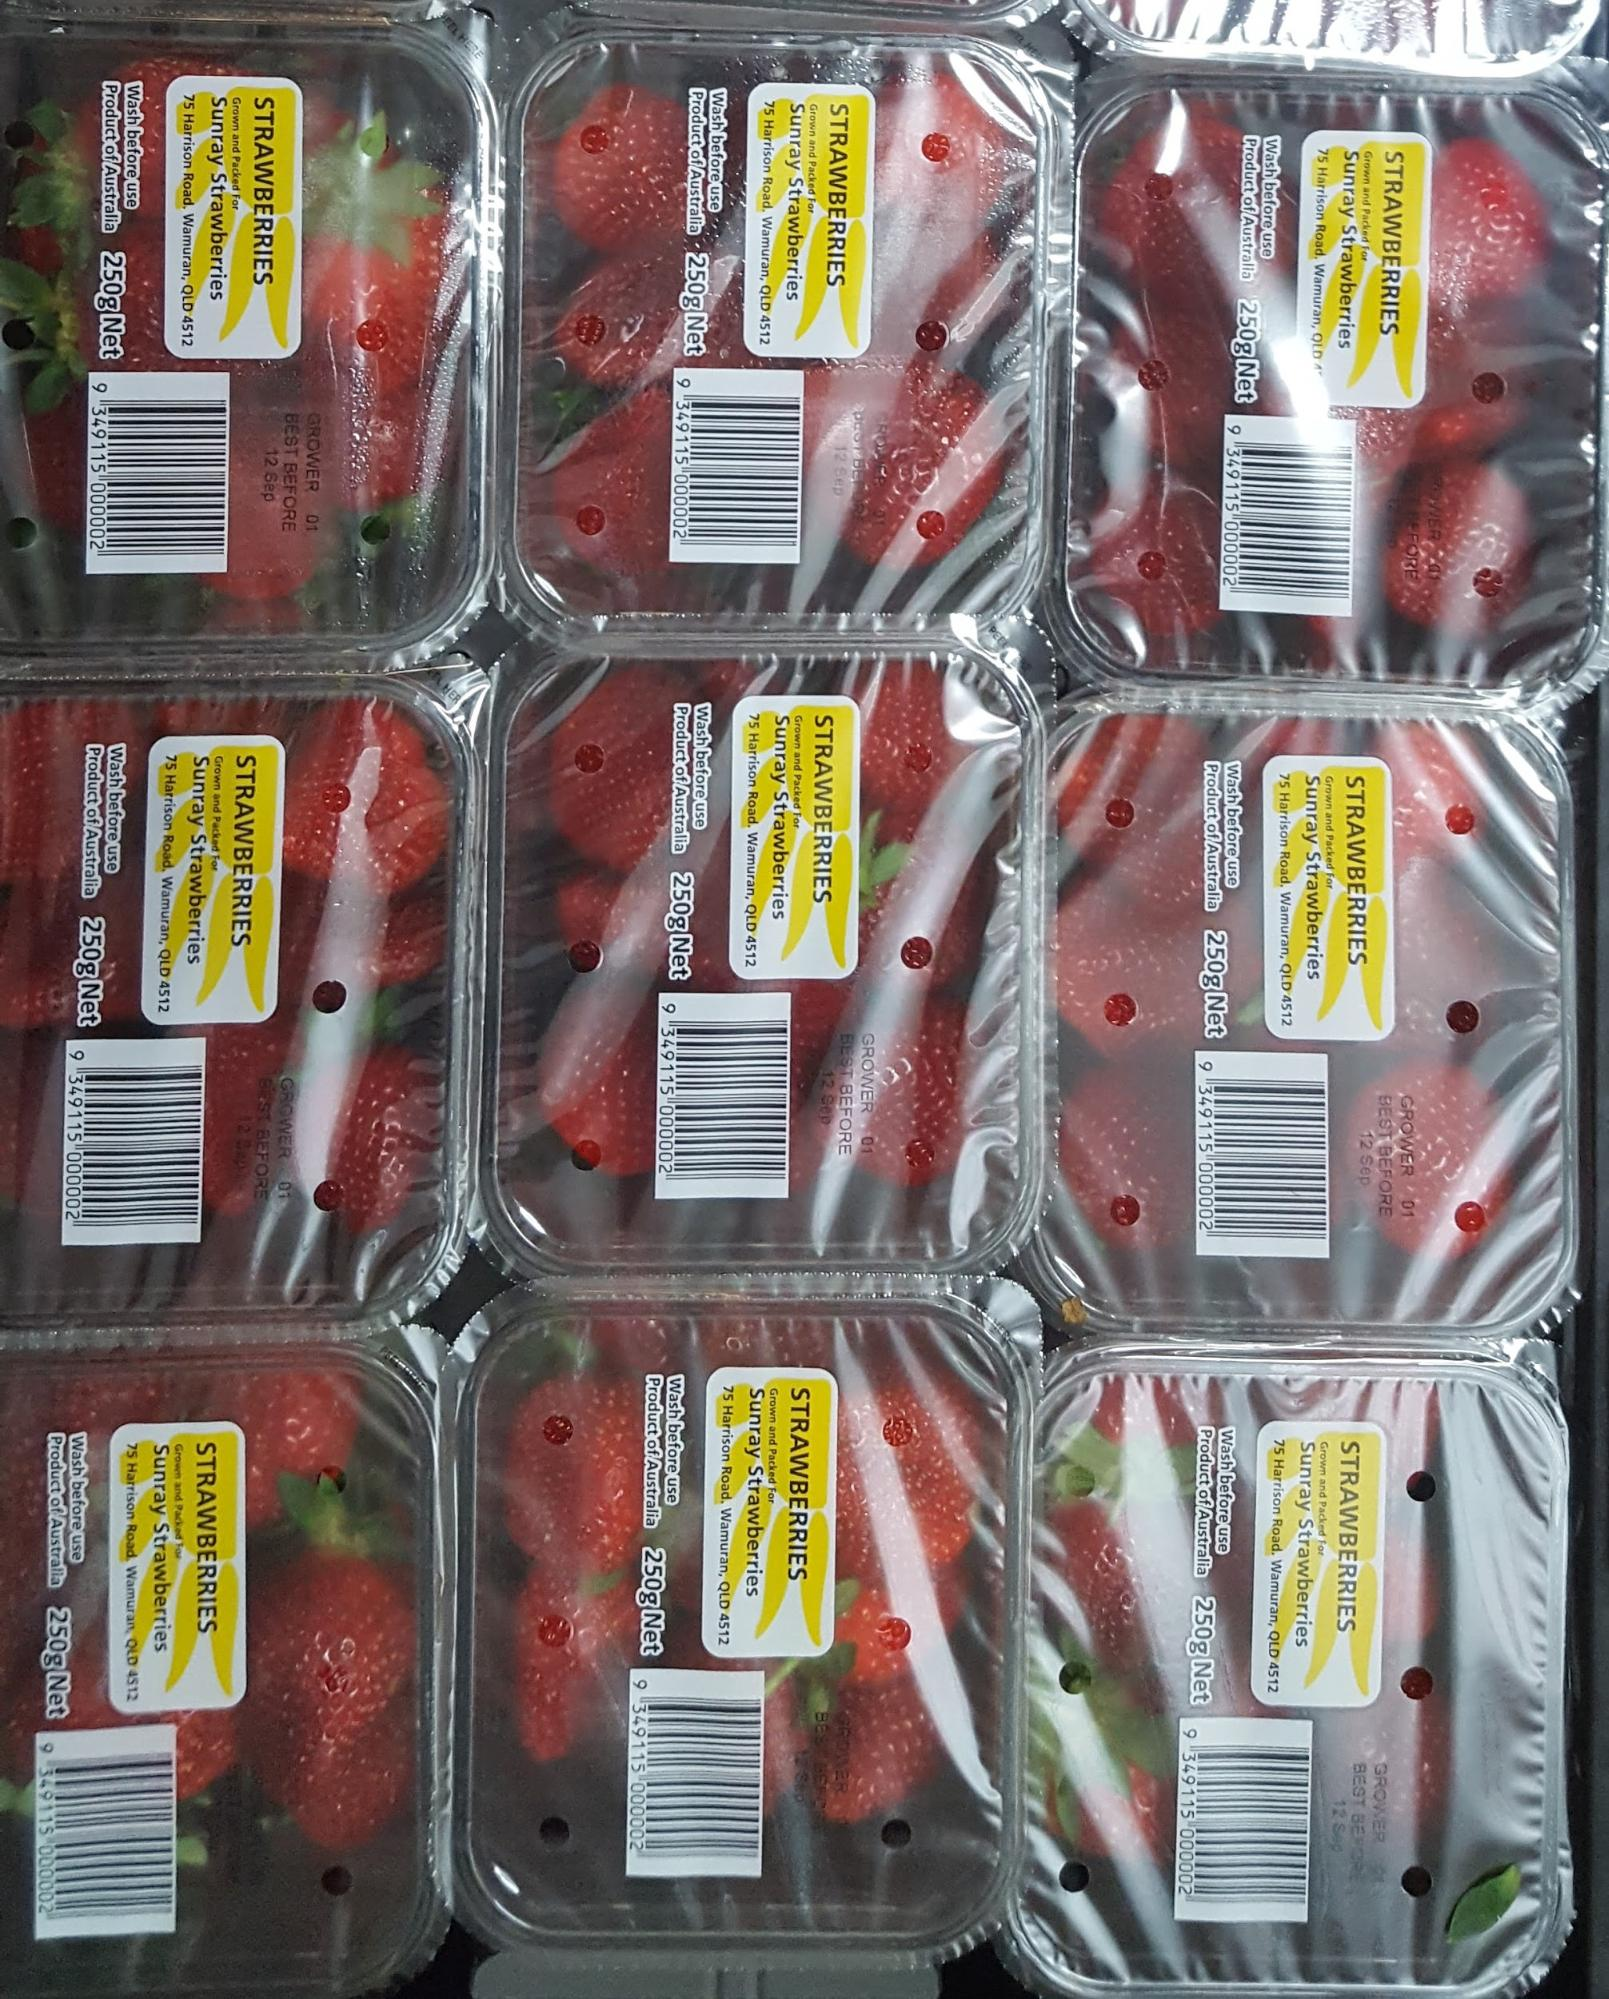
\includegraphics[width=.5\linewidth, angle=90]{sealed_punnets.jpg}
		\caption{}
		\label{fig:sealed_punnets}
	\end{subfigure}%
	\caption{(a) Heat-Seal machine, (b) Punnets before sealing, (c) Punnets after heat-sealing.}
	\label{fig:HS}
\end{figure}



Thin film rolls are used to supply the heating dye with materal to press and seal around the edge of the punnet, discarding the excess onto another roll. The pre-sealed and post-sealed punnets are shown in Figures \ref{fig:unsealed_punnets} and \ref{fig:sealed_punnets} and present a unique method to tamper-proof each punnet. The film, once removed, cannot be re-sealed giving consumers the confidence that each punnet has not been opened since it was packed. After being sealed, each item is passed through a metal detector, and a weight-checking scale. At both of these checkpoints, the punnets can be ejected from the production line using pneumatic air actuators.

Adding a vision system to the heat-seal infeed is the desired outcome for Magnificent to address quality issues that can be missed in such a fast-paced environment. Defects such as underripe, overripe, bruised, rotten, foreign object and size and shape have all been attributed to stock rejects and/or returns. Sometimes it costs more to salvage rejected stock than reuse it, so there is a possibility that poor quality could mean a shipment is subject to dumping. As millions of full punnnets are packed, palletised and shipped each year the Quality Assurance Manager has an enormous, if not imposible, task in inspecting each one thouroughly. Strawberries are required to be picked and packed to a strict set of attributes. However, subjectivity, tiredness, rushing, overheating, can all influence the quality of berries picked in the field or packed on a production line. 

Subjectivity is of great concern due to the high turnover of staff, given the majority of employees are seasonal workers, only a few of which will return each year. Therefore, the vision system will inspect each punnet from the top and bottom, at high speed, and adding objective consistency to the process as one of the final quality steps before packing.

The requirements include that the vision system feed directly into the heat-seal machine, and not inhibit the production speed or volume. This is a critical measure, particularly during development and production line integration, which ensures that efficiencies are not lost in packing. The speed of packing punnets is directly related to the profit of both the company and its workers, both of whose payments are proportional to volume over time. The company loses money paying for workers to wait for machinery to be ready, hence, downtime due to a non-critical plant will be counter-productive and should be avoided. The inspection system must be able to detect the incoming, high-speed punnets and acquire images from above and below, before analysing the quality. If the system detects defects in the strawberry images, the punnet must be removed from the production line. 


The vision system general requirements are listed in Table \ref{tab:requirements} showing other critical success factors.



\begin{table}[t!]
	\caption{Table of Requirements for Vision System.}
	\label{tab:requirements}
	\begin{tabular*}{\textwidth}{p{3cm}p{13cm}}
		\toprule
		\textbf{Requirement} & \textbf{Details} \\[8pt]
		\midrule
		\textbf{\textit{Production Line Continuity}} 	& - Shall not inhibit the production line speed. \\
							& - The production line shall not be caused to stop unnecessarily due to the vision system.\\
		\midrule
		\textbf{\textit{Safety}}    & - The vision system shall not create any safety risks or hazards such as tipping, electrocution, exposed pinch points, sharp edges, hazardous lighting, unsustainable lifting, etc.  \\[6pt]
		\midrule
		\textbf{\textit{Fruit Inspection}} 	& - Shall operate autonomously.\\
							& - Fast moving punnets shall be captured and assesed without exceptions \\
							& - The punnets shall be assesed based on the agreed defect categories (classes) to the specifications provided. \\
							& - Each punnet shall be evaluated from top and bottom (through the plastic container) \\
							& - The infeed and outfeed systems shall integrate with the proceeding and preceeding machinery. \\
		\midrule
		\textbf{\textit{Peripherals / Footprint}}	& - Shall be externally connected to one $240V$ power source, and one pnuematic line for all operations including removal from production line.  \\
		& - Shall be able to operate in any packing line given these two sources. \\
		& - Size of the system shall be kept as compact as possible due to packing line constraints. \\
		\midrule
		\textbf{\textit{Signals and Operator Information}}	& - Light and sounds shall accompany the system to be intuitive to operators \\
							& - Error, success, and general information shall be presented on a screen, or given to operators via another medium.  \\
		\midrule
		\textbf{\textit{Traceability}}		& - Records shall be kept with each punnet's images as to when (date/time) they were packed  \\
							& - Images, timestamp, assessment, system state, and other records must be kept in a database for future access. \\
		\midrule
		\textbf{\textit{Documentation}}	& - Each software module shall be documented to describe the module and it's function and relevance to the application.  \\
							& - A description of how the software is compiled and which dependencies are required to run the application shall be provided. \\
		\bottomrule
	\end{tabular*}
\end{table}






%%%%%%%%%%%%%%%%%%%%%%%%%%%%%%%%%%%%%%%%%%%%%%%%%%%%%%%%%%%%%%%%%%%%%%%%%%%%%%
%%%%%%%%%%%%%%%%%%%%%%%%%%%%%%%%%%%%%%%%%%%%%%%%%%%%%%%%%%%%%%%%%%%%%%%%%%%%%%
\newpage

\section{Current Industry Methods and Review of Literature}
\label{lab:lit}


\subsection{Image Processing in Produce Grading}

Many agricultural production lines have been adopting computer vision systems in order to reduce the cost of labor and standardise the quality control. Depending on volume, and product, quaity controllers may be a substantial cost in production and can be subjective, particularly for seasonal work.

\subsubsection{Simple Approaches}

Some simple techniques have been implemented including the work sampled by Pathare, Opara, and Al-Said \cite{pathare} in their review of colour measurment and analysis performed in order to evaluate fresh foods. They reviewed items including red table grape, tomato, orange, apple, banana, chicken breast and varied meat, flour, pasta, cerals, and breads all of which used a colour index (CI) to perform quality checks. They all had the commonality in that they used mathematical operations with co-efficients relating to one or more colour spaces such as HSV, CIE-Lab, and CIE-XYZ. These colour indexes were used to make a comparison against test samples for characteristic representation of maturation, preservation, or storage. Sandrina et al \cite{sandrina} implemented a method using geometric calculations to determine weight and shape of watermelons. Using logistic regression analysis they determined that good specimen shape could be well-described by an ellipsoid model with an $R^2$ of $0.97$. The weight of the watermelons was estimated by image analysis with an error of $2.42\%$. In order to grade palm oil fruit, May and Amaran \cite{may} simply analysed the RGB range of underripe, ripe and overripe fruit colour and determined accociated values correlating to the ripeness. Their fuzzy logic system achieved an overall accuracy of $86.67\%$ showing that this method is plausible for fruit ripeness determined by colour. A method to grade four different varieties of mango into four ripeness grades was implemented by Nandi, Tudu, and Koley \cite{nandi} by extracting colour features, and deriving other colour features at key points across length of the fruit. The features were then used with a simple Gausian Mixture Model (GMM) to achieve accuracies that rivaled expert humans. Hasan and Monir \cite{hasan} developed a system to evaluate guava by use of a Fuzzy Inference System (FIS). The fuzzy rules were based on functions of hue, saturation, and intensity of the images acquired of the fruit. Their method achieved an accuracy of $93.4\%$ which is an improvement over other classifiers such as naive bayes and multi-SVM. A method to grade lemons based on colour and volume was implemented by Khojastehnazhand, Omid, and Tabatabaeefar \cite{khojastehnazhand} where the system could be calibrated to the specific requirements before assessment begins. By passing through fruit as examples to the system (and stored in a database), before using the example data as comparrison to the unseen fruit. The colour and volume information was calculated via HSI colourspace and simple geometry measurements where the volume estimation $R^2 = 0.9852$ and colour (ripeness) estimated accuracies of $95.45\%$, $100\%$, and $86.67\%$ for classes 1, 2, and 3, respectively. Blasco, Aleixos, and Molto \cite{blasco2} developed an algorithm that can detect 12 different types of common disease in citrus fruits. The method could assess fruit from different batches, and even species, of citrus without adjustments by using a region-growing technique based on the assumption that unaffected fruit peel is relatively consistent, smooth, and blemish-free. An overall accuracy of $94\%$ was attained with some of the most devastating diseases scoring $100\%$ detection.





\subsubsection{Pysical}

Chui et al\cite{chiu} used a process of acquiring flourescence images - exiting the internal structure of the object in one wavelength, to emit light at a different wavelength - in order to detect mechanically-induced bruises on apples. They found that this method highlighted the bruised flesh, and extracted them by performing an image difference with a local adaptive binarisation method. Matteoli et al \cite{matteoli} used a fibre-optic spectrometer to take measurements of peach fruits whilst performing destructive density testing in order to make predictions on new fruit non-destructively. They compared the output of a crisp versus fuzzy logic approach and found overall average accuracies of $60\%$ and $~80\%$, respectively, making the fuzzy system appropriate for the task. Choi et al \cite{choi} also used an NIR spectrometer to assess the internal qualities of pear fruit as well as CCD cameras to inspect the visible characteristics such as skin blemishes and colour. The spectroscope analysed the fruit for sweetness, acidity, hardness, and moisture before combining the two (visible and internal) features as classification variables for an ANN. A method that used volumetric estimation in order to perform quality grading in fruit (apples, mango, orange, pomegranate, and strawberry) was designed by Jadhav, Singh, and Abhyankar \cite{jadhav}. Four cameras positioned at various angles and elevations were used to acquire the callibrated images of fruits before the volumetric calculations were peformed. This information is coupled with the colour values from the hue channel of HSV colour space to obtain a classification grade which is then passed to a Fuzzy Inference System (FIS) for final distribution into five grades from very poor to very good. All grades and all fruits achieved accuracies of $>98\%$.  



\subsubsection{Hand-selected Features}

Hand selecting features is a common approach to help classifiers or networks to focus on the most important characteristics which determine class or defect. A tomato maturity level grading system developed by Wan et al \cite{wan} by projecting 5 concentric circles with different radii onto the fruit in order to extract the colour feature value. The correlated hue values were used to represent the maturity level before being trained on a 3-layer BPNN, achieving an average accuracy of $99.31\%$. Pereira et al \cite{pereira} hand crafted 21 colour features utilising three colour spaces (RGB, CIE-Lab, and HSV) in order to grade papayas into three maturity stages (MS). The mean values, pixel areas, and differential indexes between these colour spaces were obtained and classified by Random Forrest method resulting in an accuracy of $95.4\%$, $92.1\%$, and $84.4\%$ for MS1, MS2, and MS3, respectively. The team noted that it may be suitable for an industrial application in future. Mebatsion, Paliwal, and Jayas \cite{mebatsion} found the best results when pairing morphological features with colour features in order to classify cereal grains into five common categories. They used a simple least-squared classifier obtaining a result of $98.5\%$ for barley, $99.97\%$ for CWRS (Canada Western Red Spring), $99.93\%$ for oat, and $100\%$ for rye and CWAD (Canada Western Amber Durum). Szczypinski, Klepaczko, and Zapotoczny \cite{szczypinski} used an ANN classifer to attempt to discriminate between 11 different barley strains. 13 statistical metrics were obtained such as mean, skewness, second moment, and entropy in order to differentiate the varieties with an accuracy ranging $67\%$ to $86\%$. In an effort to grade persimmon fruit into three commercial maturity stages, Mohammadi, Kheiralipour, and Ghasemi-Varnamkhasti \cite{mohammadi} extracted features relating to RGB, CIE-Lab, HSV, and greyscale conversions before training both an LDA and QDA classifier to perform the categorization. The QDA model achieved an overall accuracy of $90.24\%$. Muhammad \cite{muhammad} also used hand-selected features when developing a method to classify date varieties. After an ellipse has been fit to the date image, features such as major and minor axis length, eccentricity, area, and texture descriptors were extracted and trained with an SVM classifier to achieve accuracies of $100\%$, $96.2\%$, $96.6\%$, and $99.6\%$ for the four varieties analysed. Selected features chosen by Thendral and Suhasini \cite{thendral} improved the results, compared to no feature selection, for all tests performed whilst detecting defects in orange peel. They compared the performance of SVM, BPNN, and AANN finding that the AANN delivered the best testing results of $94.5\%$. Gill, Girdhar, and Singh \cite{gill} used a hybrid intelligent solution when developing a fruit grading method by means of a Genetic Algorithm merged with BP-ANN. The Back-Propagating (BP) method used to update weights in the network has a tendancy to become trapped in a local minima, leading to the idea of genetic algorithm (imitating natural evolution) coul overcome this problem. The results indicate that the hybrid system has increased accuracy ($93.33\%$) compared to a conventional BP-ANN ($73.33\%$).  









\subsection{Strawberry Image Processing}

Brosnan and Sun \cite{brosnan} performed a review of agricultural vision systems including apple grading, orange stem detection and sweetness correlation, unsplit pistachio nuts, tomato size, colour, and shape properties as well as seedling health, peach and pear maturity levels, and automatic fruit harvesting. The team also reviewed vegetable inspection methods such as musshrooms and potatos, as well as wheat, rice and corn. The team noted 2 methods for analysing strawberry shape and size, taking one of the teams $1.18 s/berry$ and noting that fruit quality is dependant on a number of pre-harvest and post-harvest processes. Liming and Yanchao \cite{liming} developed a strawberry grading method and mechanical system that requires manual loading of single strawberries on a converyor belt before using colour features and k-means clustering to grade the fruit into shape and colour classes at a rate of approximately $2.5s/berry$. Cubero et al \cite{cubero} reviewed Apple, banana, citrus, cucumber, mango, mushroom, olives. potatoes, starfruit and watermelon as part of their investigation into agricultural machine vision. Methods such as colour analysis, histogram, k-NN, PCA, Fourier analysis, clustering, AdaBoost, and ANN's to perform the tasks of inspecting a wide range of defects and classifications. Another review by Dubey and Jalal \cite{dubey} investigated two types of tasks for vision systems - classification and defect detection - and concluded that most of the work in this field contained three steps in performing either task, namely, 1. Background subtraction 2. Feature extraction and 3. Training and classification. SVM, BPNN, Decision Tree, ANN, and even fusion classifiers were commonly used in their research. Strawberry cultivar are numerous around the world and their distinguishing features seem only obvious to expert humans as shown in K. Yamamoto et al \cite{yamamoto} when they implemented a method to distinguish between 21 different strawberry cultivars. They found that when using a single feature such as colour, shape, or size, the average accuracy was very poor at $<42\%$. However, when these three features were used in conjunction, the discriminant analysis classifier performed better at $68\%$. This shows that strawberry cultivars are not simply classified. S. Yamamoto et al \cite{yamamoto2} used simple RGB techniques to define the ripeness of strawberries whgen developing an automated harvesting machine. They used a combination of green, red, and white LED's in order to illuminate the strawberries in specific wavelengths, giving better judgement on whether to pick or not based on ripeness. The harvesting machine was designed to be stationary with the fruit being presented to the machine via moving beds, which implies a large amount of fabrication and process chgange would be required to persue this method. The authors reported high harvesting rates ($67.1\%$) compared to that of other more conventional harvesters, however, their system was succeptible to fruit damage and requires improvement in harvesting speed.


\subsection{Real-time Systems}



Sofu et al \cite{sofu} designed and automatic apple sorting system which processed at a rate of $54,000 apples/h$ acheiving an accuracy of $79\%$. A simple descision tree was used to classify the specimens according to colour, size, stain and weight before sorting the apples using opening bowl mechanisms. A fig sorting system developed by Baigvand et al \cite{baigvand} could successfully categorise the figs into five grades with accuracies up to $95.2\%$, processing at a rate of $90kg/h$ and sorting each into separate bins using air nozzles. The team created indices related to colour, size, and the area of the split, seen on each fruit, applying a rule-based method to determine the graded category. Lee et al \cite{lee} implemented an industrial date grading machine capable of processing $72,000 dates/h$ with an $87\%$ accuracy measured. They acquired images in NIR wavelengths ranging $750-1200nm$ by use of an NIR-extended CCD camera and a high pass filter to block wavelengths lower than $750nm$. This provided good background segmentation, added to the amplification of delaminated skin features which determine quality. The amount of delaminated skin was calculated, after morphological operations, and compared to the size of the entire fruit to give a percentage and a grade from A-E. 



\subsection{Machine Learning / Deep Learning Methods}

Zhang et al \cite{zhang} used an FNN to classify a fruit dataset created via on-site collection and on line. After background removal, the 79 features that had been constructed based on colour, texture, and shape were obtained before being reduced via PCA to 14, and used to train the network using 5-fold cross validation. The classification accuracy of $89.1\%$ outperformed other methods tested such as BP, momentum BP, and GA. Zuniga et al \cite{zuniga} used a supervised learing approach with small neural networks in order to grade grape seeds from images acquired scattered over a flat-bed scanner. Using a process of analysis and trial and error, the optimal number of neurons is found and a classifier trained giving total accuracy of $86\%$ for the test set. An SVM classifer trained by Sabri et al \cite{sabri} was able to classify ripe and unripe palm oil fruits with an accuracy of $96.59\%$. They compared three methods of feature extraction (Colour histogram, colour moment, and colour correllogram) and two classification methods (SVM and Naive Bayes) in order to find the best results with SVM prevailing. However, SVM was not the predominant classifier when Alfatini et al \cite{alfatni} designed a palm oil grading application. The method consisted of using a basic grey level aura matrix (BGLAM) technique to extract features followed by an ANN classifier. After assessing ANN, KNN, and SVM classifiers, the best results were realised using the ANN with accuracy of $93\%$ and speed of $0.4s$. An ANN was also used by Bhatt and Pant \cite{bhatt} when grading apples based on size, colour, and external defects. Seven selected features were used (3 colour features, 1 size, 1 damage, 1 symmetry, and 1 weight) to train the ANN achieving $90\%$ testing accuracy. An apple grading system developed by Vakilian and Massah \cite{vakilian} used a 3-layer ANN whilst grading Golden Delicious and Red Delicious varieties with respective overall accuracies of $89\%$ and $92\%$. Extracting the images textural (mean and variance of energy values) features before training separate networks for each apple variant. Finally, they invstigated the width of the ANN's middle layer ranging the architechture of the network from $2-2-4$ to $2-20-4$ finding the optimum width of $2-12-4$. 


Wang et al \cite{wang} whilst developing a method to find worm-eaten holes in chestnuts. Using Sobel edge detection and using the resulting, filtered region to train a BP network. Conversion occured after only three iterations and achieved $100\%$ for both good and wormhole classes. 



For an activation function $f$, the $i^{th}$ neuron $a$ is given by:
\begin{equation}
	a_i = f\bigg((w_i^0 x_i^0 + b_i) + (w_i^1 x_i^1 + b_i) + (w_i^2 x_i^2 + b_i) + ... + (w_i^n x_i^n + b_i)\bigg)
\end{equation}

giving 
\begin{equation}
	a_i = f\bigg\{b + \sum_{i=0}^{n} w_i x_i \bigg\}	
\end{equation}




\subsection{Control Systems}

Vision systems have been utilised on many production lines since the early 1980's \cite{kruger}. Computers represent a medium to perform a consistent, verifiable approach to monitoring, recording, and quality control of produced items. These items may be susceptable to damage, contamination, manufacturing errors, poor quality, out-of-specification features, or defects and require separation from good quality produce. Depending on the goods being monitored, there may be an option to rework, correct, repack, or remake the defected instances, therefore, the control systems will differ greatly between production lines.   

The fruit grading system by Kondo \cite{kondo} used two robot arms with 3 DOF performing a series of tasks to determine colour, size, shape, and defect. The robots alternate using suction cups to pick up 12 fruit at once in order to acquire images from the above, below, and 4 sides before pushing them into the corresponding lines. 12 camera systems in total are used, with others guiding the manipulators. This, and the project by Michalosa et al \cite{michalosa} combining mobile robots with tooled manipulators serves as examples of precision, complex, robotic control systems. However, as agricultural production line items generally are not required to be assebled or involve precise movements, control systems are relatively easy to implement, without the need for complexities such as several degrees of freedom or specialised tooling to perform the task of quality control.  

Blasco et al \cite{blasco} performed grading of pomegranite arils into five categories - White, Pink, Red, Brown , and Unwanted using several pnuematic air nozzles to eject the arils into their appropriate outlets. The system can grade a maximum of $75kg/h$ using six narrow conveyors and is highly dependant of the feeding unit to uniformly distribute the arils on the conveyor belts. As the air nozzles have a conical burst of air, incorrect rejections can occur if they are too closely distributed, or if external factors cuase the arils to roll between the vision system and control. Pneumatic air ejectors helped Nouri-Ahmadabadi et al \cite{nouri-ahmadabadi} in order to grade pistachio kernels from unwanted shells. The system also required a good separation of individual items on the conveyor in order to correctly eject the affected instances. The sorter requyired an $8mm$ separation and could process $22.74kg/h$ with an accuracy of $94.33\%$. A date grading system by Al Ohali \cite{ohali} used electro-mechanical sorting strips placed at the end of the conveyors which guide the fruit into different grades. This type of control must have even larger spacing due to the mechanical movement followed by a return. Systems developed such as Sa'ad et al \cite{saad} mango shape and weight grading project used push/pull actuators to remove defect items and is akin to conveyor process control (i.e. conveyor separation, interleaving conveyors, conveyor gates, etc). Makky and Soni \cite{makky} developed a grading machine for oil palm fresh fruit bunches using stepwise discrimination in order to classify into accept and reject classes with an average success rate of $93.53\%$. Their design (and in-field implementation) employed a gate driven by a limit switch to separate the good fruit from the rejected.




%%%%%%%%%%%%%%%%%%%%%%%%%%%%%%%%%%%%%%%%%%%%%%%%%%%%%%%%%%%%%%%%%%%%%%%%%%%%%%
%%%%%%%%%%%%%%%%%%%%%%%%%%%%%%%%%%%%%%%%%%%%%%%%%%%%%%%%%%%%%%%%%%%%%%%%%%%%%%
\newpage

\section{I - Prototype and Research}

\subsection{Design and Construction}








\begin{figure}[h]
	\centering
	\begin{subfigure}{.4\textwidth}
		\centering
		\includegraphics[width=.6\linewidth]{top_bottom_lights.jpg}
		\caption{}
		\label{fig:enclosure_1}
	\end{subfigure}%
	\begin{subfigure}{.6\textwidth}
		\centering
		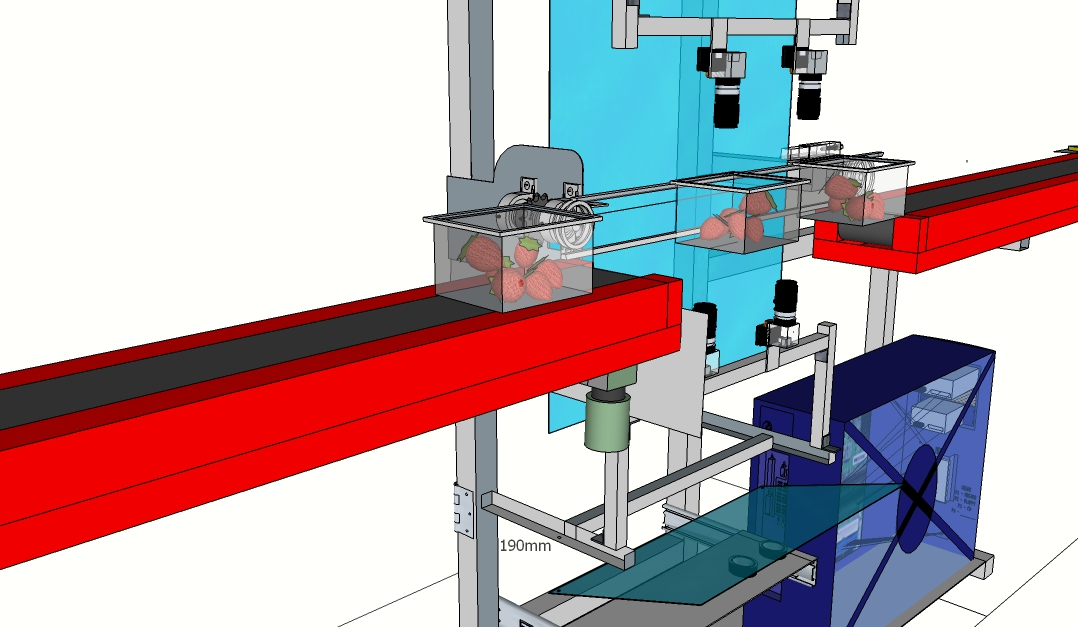
\includegraphics[width=.8\linewidth]{QAS_cross_sec.jpg}
		\caption{}
		\label{fig:cross_sec}
	\end{subfigure}%
	\caption{(a) The frame of enclosure shown with sheetmetal wrapped around to form the enclosure. (b) Cross section of the enclosure schematic.}
	\label{}
\end{figure}






\subsubsection{Specular Reflections}


\begin{figure}[h]
	\centering
	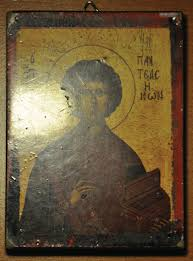
\includegraphics[width=200pt]{images/specular_art.jpg}
	\caption{An image of an painting with a large specularity occluding the image.}
	\label{fig:specular_art}
\end{figure}

This is due to Snell's law which states,
\begin{equation}
\eta_{1} sin\theta_{1} = \eta_{2} sin\theta_{2}
\end{equation}

and when the mediums $\eta_{1}$ and  $\eta_{2}$ are the same or equal it can be seen that,
\begin{equation}
\theta_{i} = \theta_{r}
\end{equation}

where $r$ the reflected wave, has at the same angle as $i$ the incident wave from the normal of the surface. 



There are a few methods to combat the specular reflections, such as polarizing the light, changing the angle of the source, or diffuse lighting. In the case of this project, all three are implemented in order to reduce the specularities to a minimum.

Polarization of a light source, using a polaroid sheet, will reduce the overall light intensity by a factor of $\frac{1}{2}$ due to Malus' law given by
\begin{equation}
	I = I_{0} cos^{2}\theta_{i}
\end{equation}

with $I_{0}$ being the initial intensity and $\theta_{i}$ is the angle of the polarizer axis from the angle of initial polarization. If a light source is unpolarized, it is thought to have a combination of all polarization directions and so $cos^{2}\theta$ is averaged to $\frac{1}{2}$. Although, in practice, this figure is less than this due to imperfections in polarizing material and, hence, more light will be required in order to achieve the same luminosity on the subject \cite{rox, sommer}.



\begin{figure}[h]
	\centering
	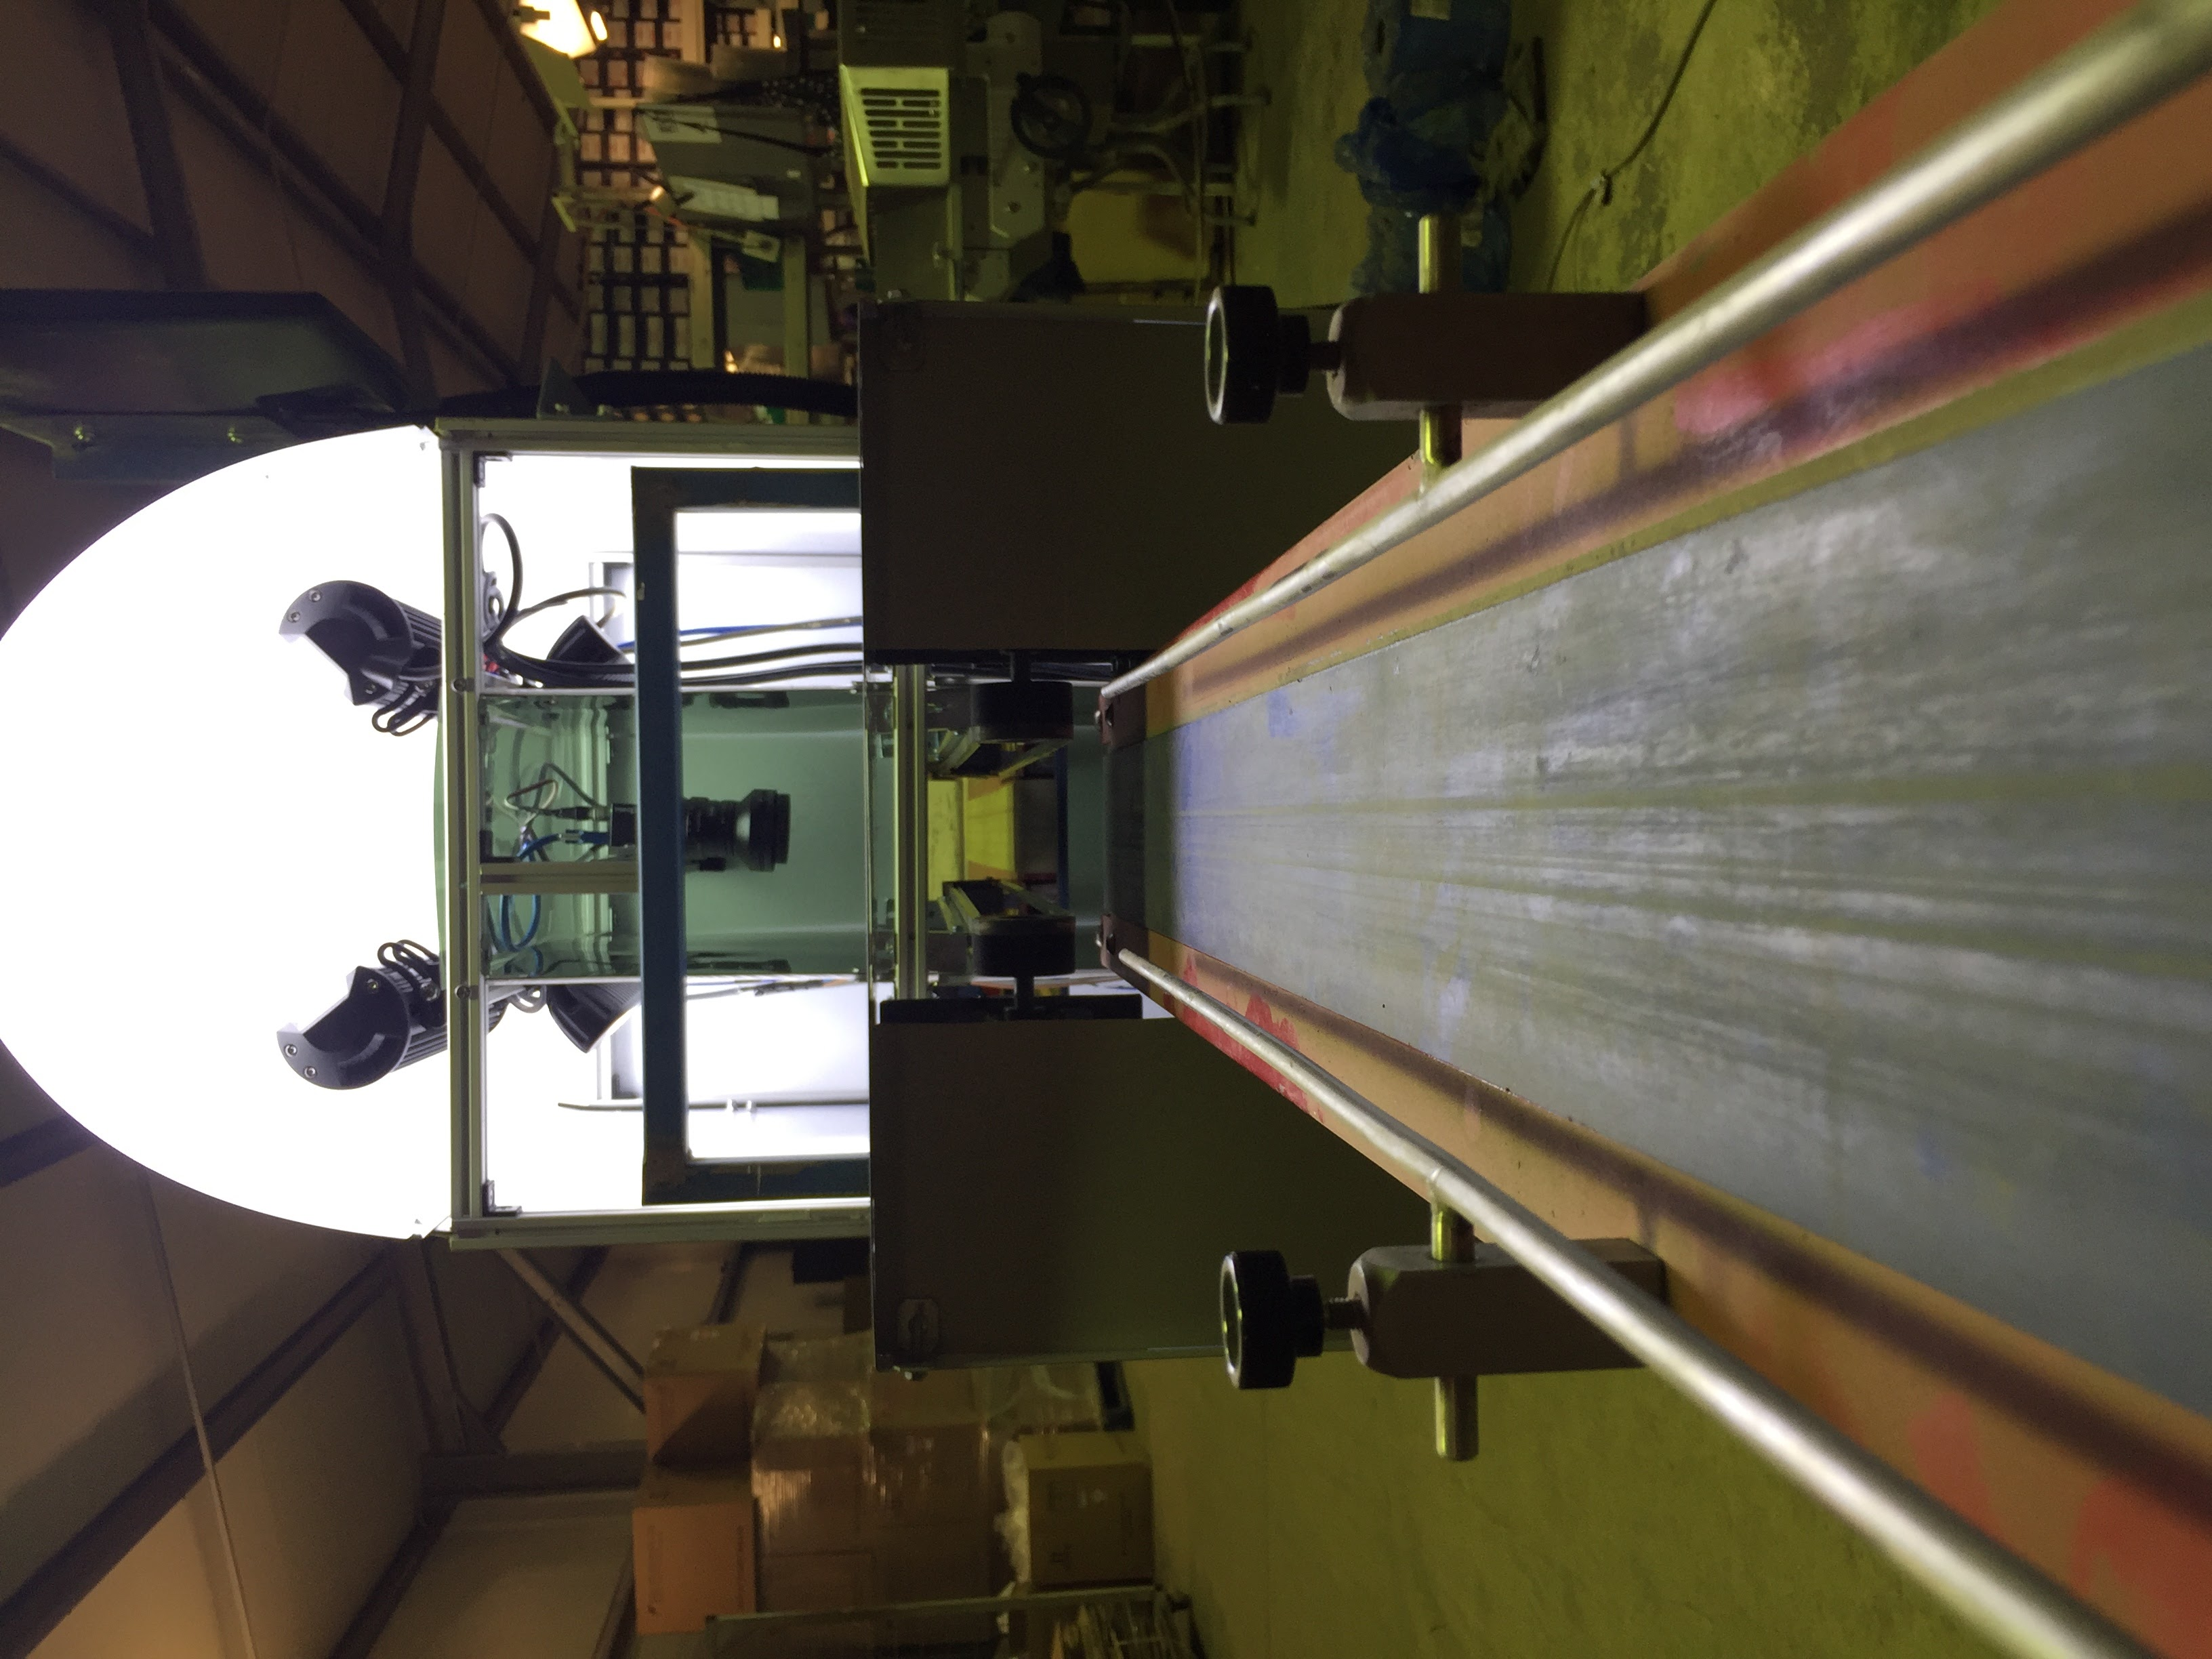
\includegraphics[width=300pt]{images/enclosure_3.jpg}
	\caption{Looking through the enclosure in the path of the punnet, the cameras are mounted inside the polarized and difuse chamber as the v-belts transfer the punnets unobscured through the enclosure. Note: front panel removed to show arrangement.}
	\label{fig:enclosure_3}
\end{figure}





\subsection{Electronics}



\begin{itemize}
	\item PC for image processing and control of devices and hardware
	\item Lighting for illumination
	\item Cameras to capture images
	\item Punnet sensors
	\item Microcontroller for hardware operation
	\item Relay bank to switch high-power sources
	\item Peltier devices
	\item Uninterruptable Power Supply (UPS)
	\item Intake/exhaust/cooling fans
	\item Various circuits/wiring/connectors/fuses
\end{itemize} 




\subsubsection{Power Requirements}


\begin{table}[h]%
	\caption{Power requirements for the electronics used in the system.}
	\centering
	\includegraphics[width=0.9\textwidth]{images/power_req.png}
	\label{tab:power_req}
\end{table}



\begin{figure}[h]
	\centering
	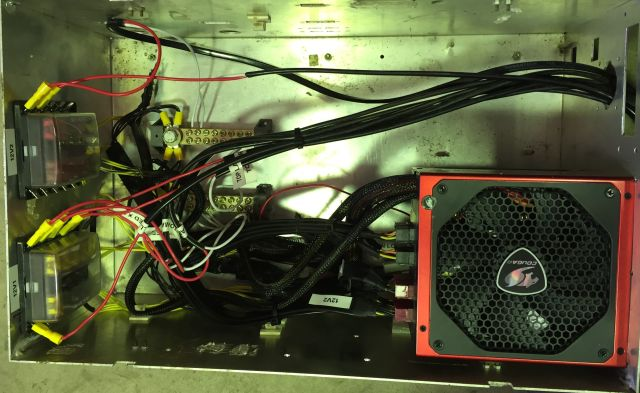
\includegraphics[width=0.8\textwidth]{images/PSU2.jpg}
	\caption{Power Supply box with PSU mounted, fuses, ground terminals, and wiring to the electronics throught upper right wall.}
	\label{fig:PSU2}
\end{figure}




\subsubsection{Hardware}



\begin{figure}[h]
	\centering
	\includegraphics[width=\textwidth]{images/overview.png}
	\caption{Overview of the electrical connections and control hierarchy of the SQA system.}
	\label{fig:overview}
\end{figure}  




\subsection{Software}



\subsubsection{User Interface}




\begin{figure}[h]
	\centering
	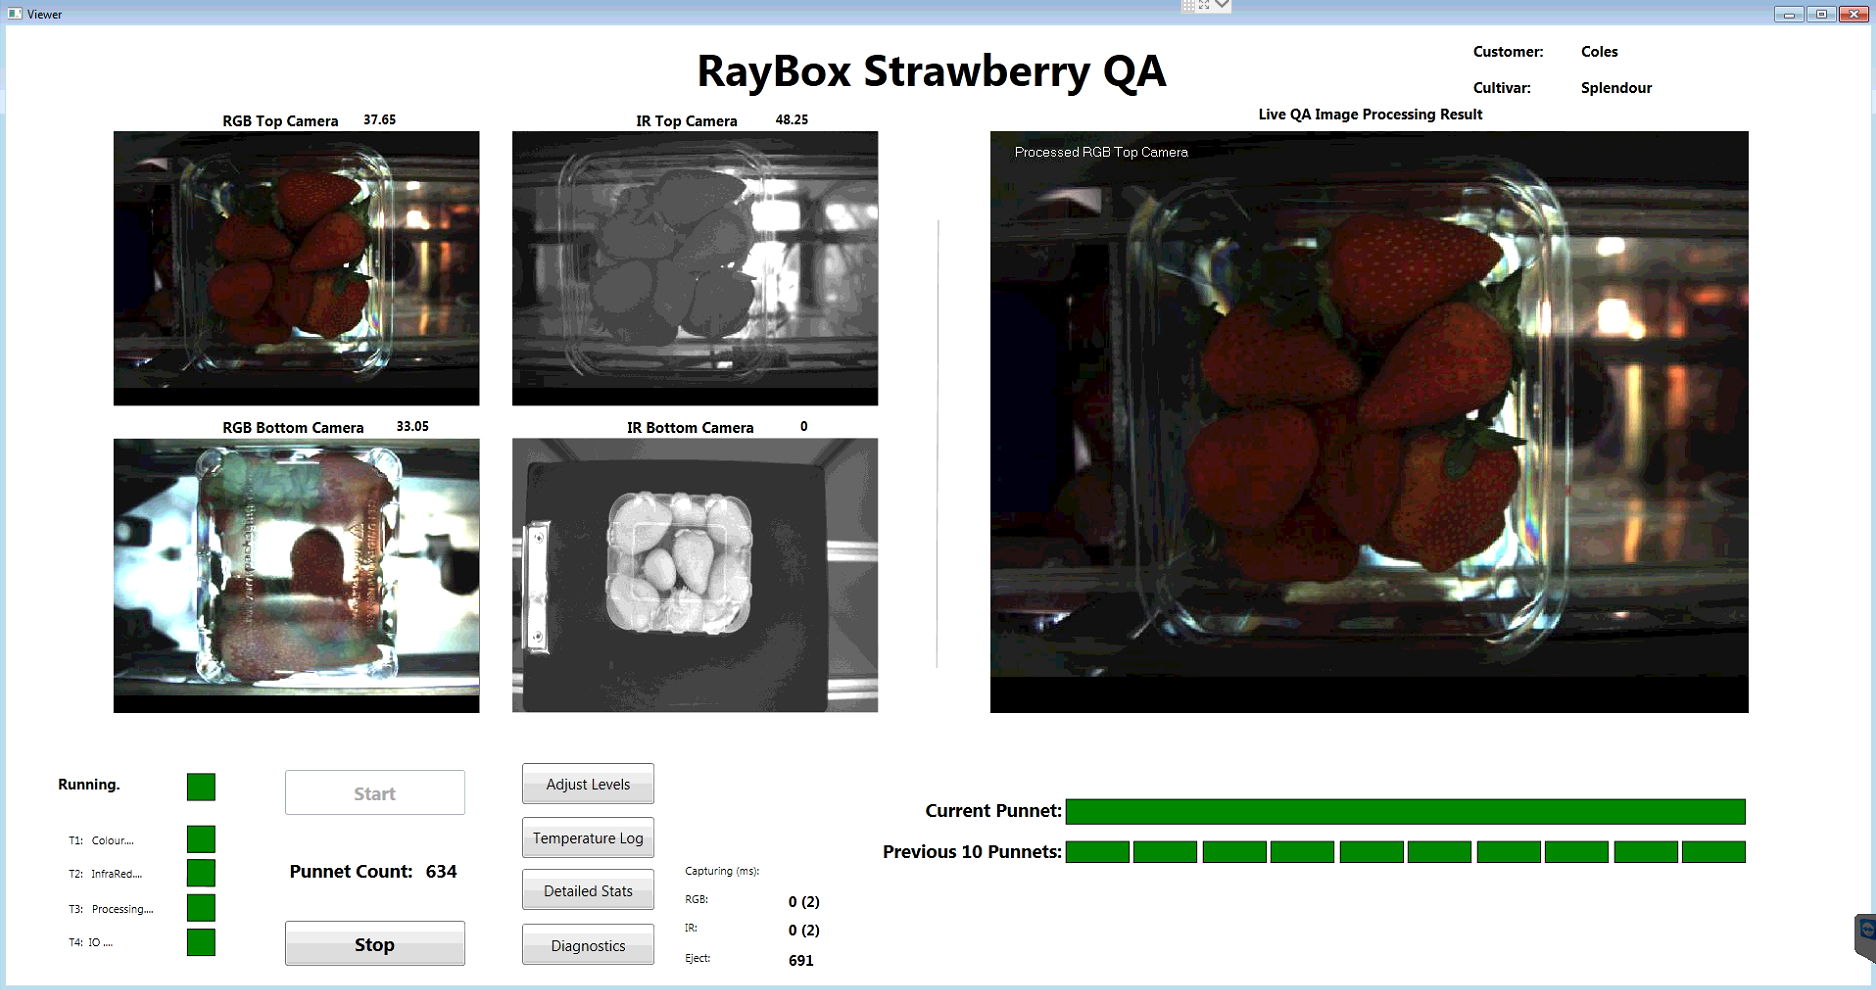
\includegraphics[width=0.7\textwidth]{images/GUI.png}
	\caption{GUI for the SQA vision system.}
	\label{fig:GUI}
\end{figure}
  


\subsubsection{Asynchronous Grabbing}




\begin{figure}[p]
	\centering
	\includegraphics[width=0.9\textwidth]{images/software_flow.png}
	\caption{Flow chart of the main application with each of the five threads (including main) and thier progress reporting.}
	\label{fig:software_flow}
\end{figure} 




\subsubsection{Hardware Control}

Various hardware devices will need to be controlable via the main application, to enable efficient main lighting, signal lighting, peltier, pneumatics, and conveyor control, as well as inputs from some peripheral devices and sensors.

The \texttrademark Phidget is an industrial-style microcontroller with integrated I/O that can be interfaced with a PC and has strong electrical connectors. An advantage of this microcontroller is that it can be programmed in $C\#$ programming language, therefore interfacing with the main application will be simplified. 

\begin{wrapfigure}{r}{0.5\textwidth}
	\begin{center}
		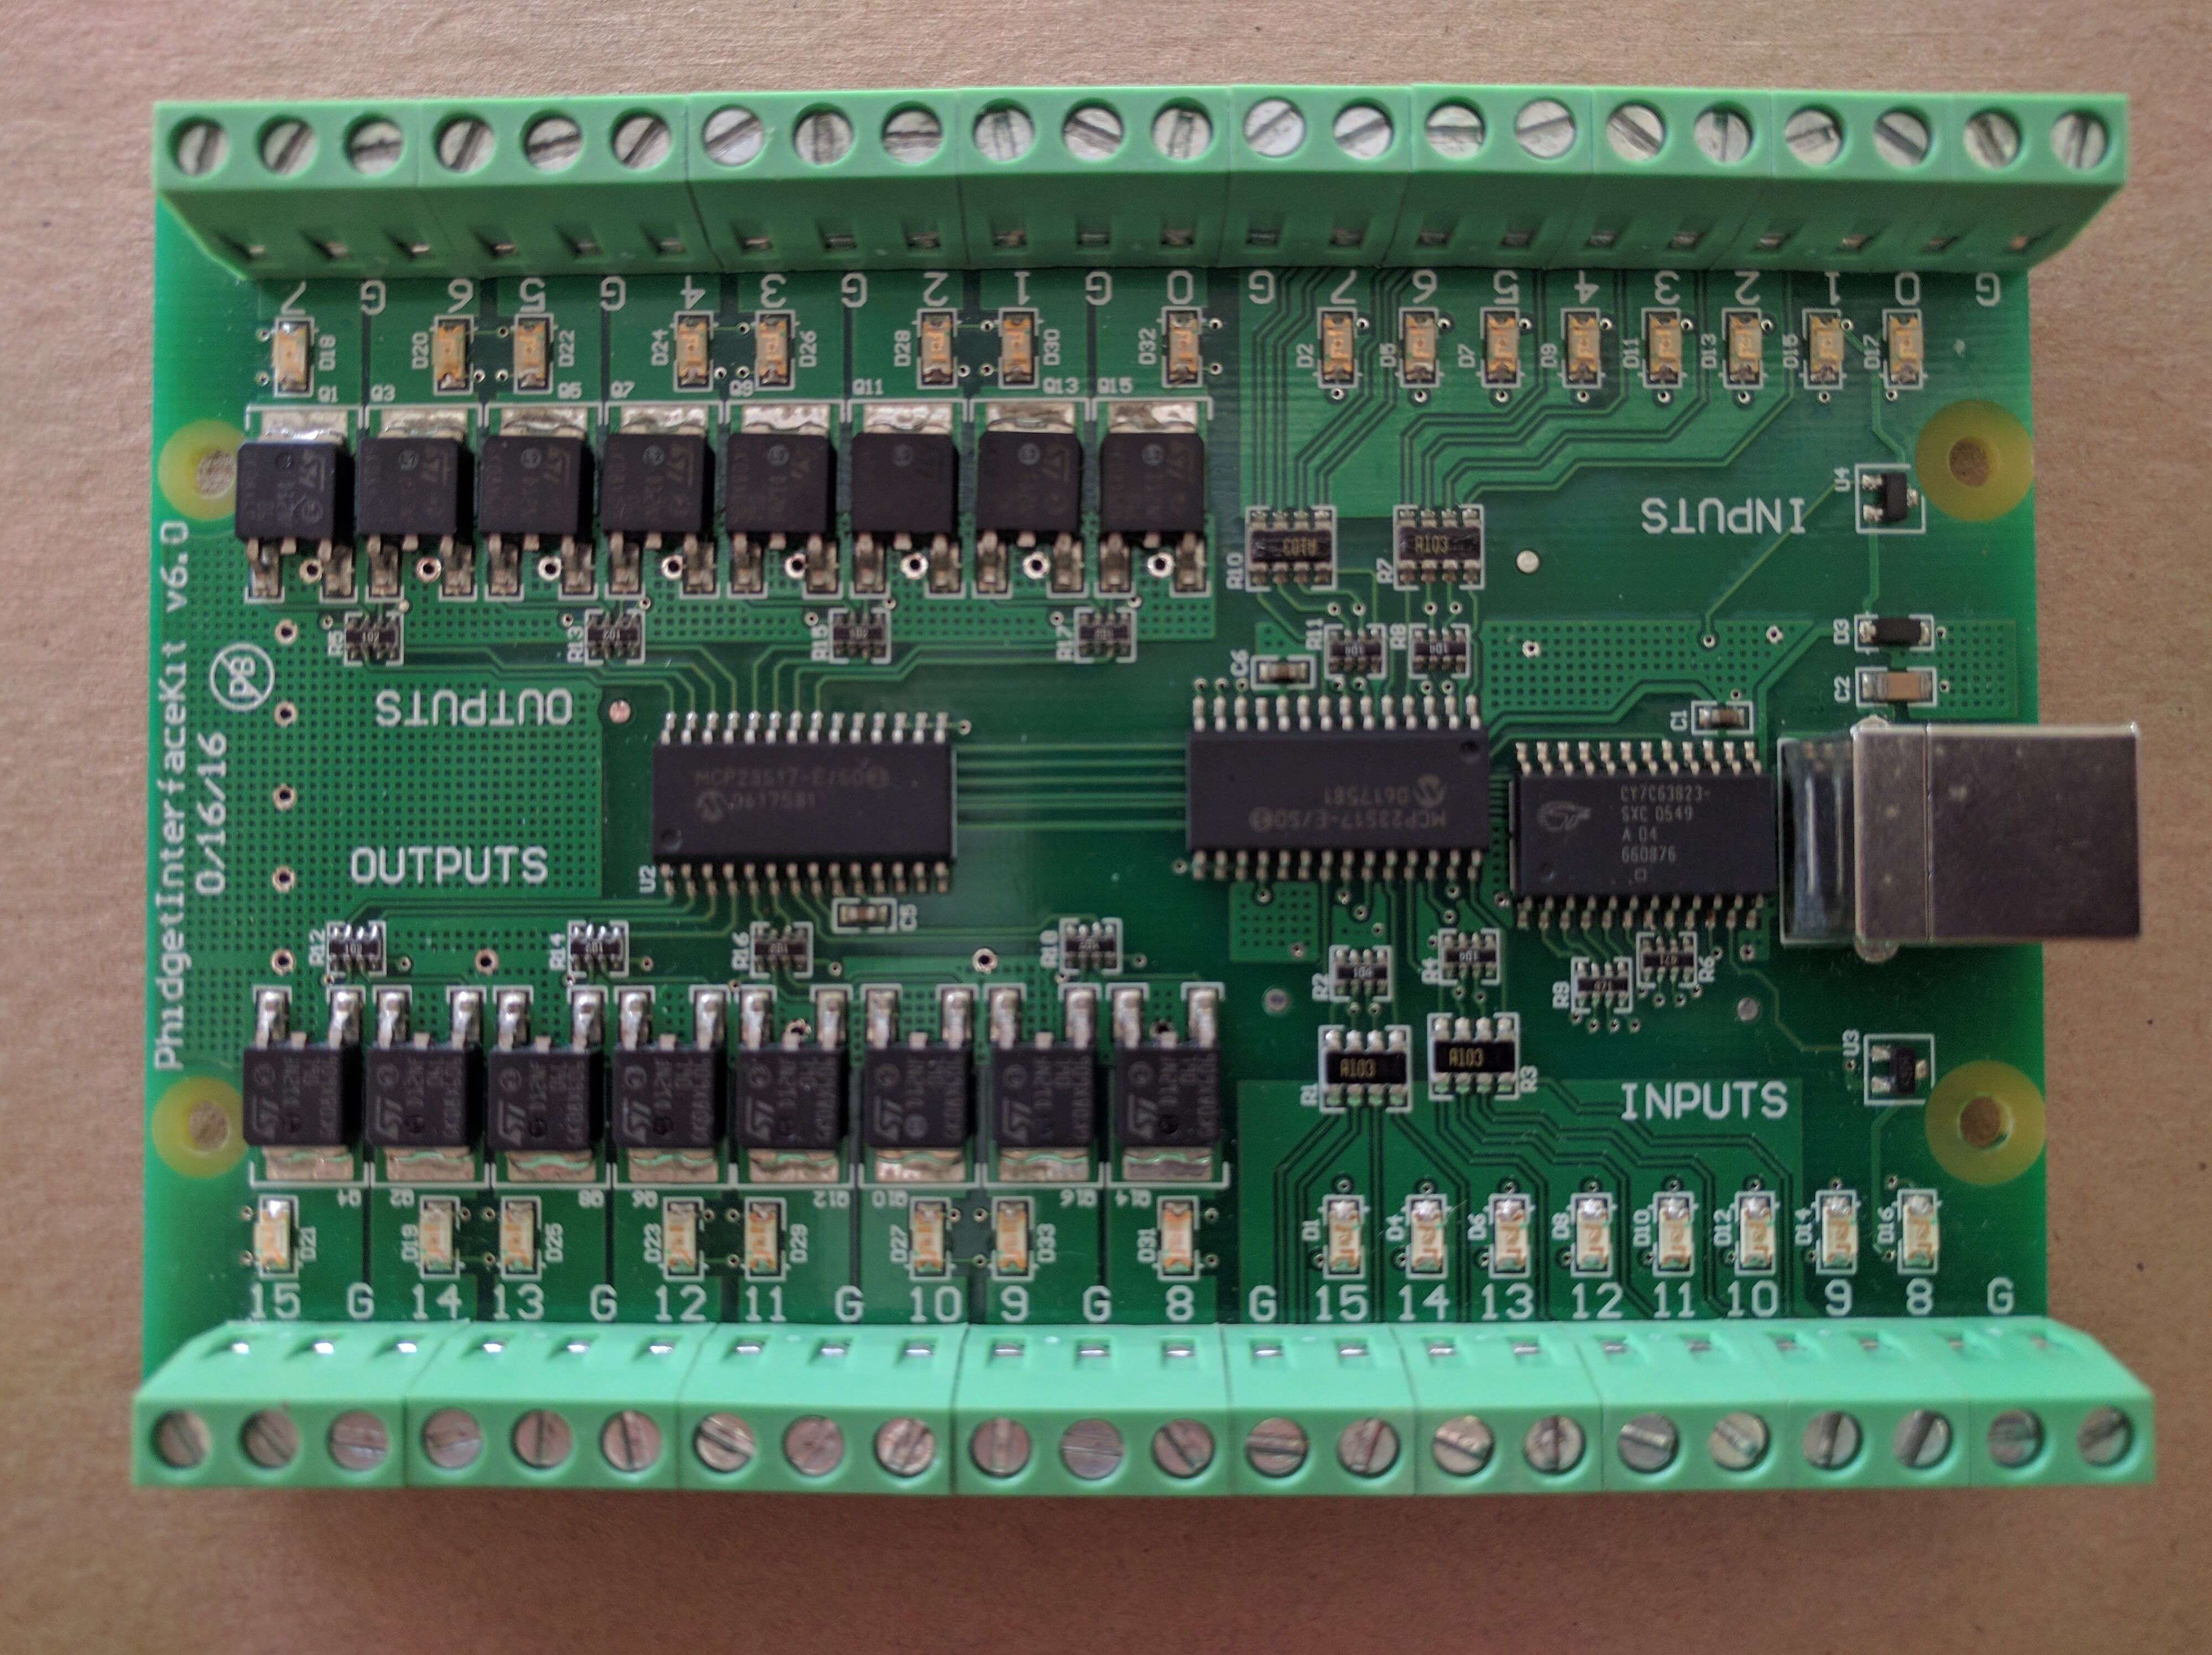
\includegraphics[width=0.5\textwidth]{images/phidget.jpg}
	\end{center}
	\caption{Image of the Phidget \texttrademark I/O board and the interface connectors on the top and bottom.}
	\label{fig:phidget}
\end{wrapfigure} 

The Lighting must be only turned on when in operational mode, therefore, the power is switched through a relay bank with the Phidget operating as the controller, as described earlier in figure \ref{fig:overview}. This will save energy and lengthen the lifetime of the lighting, as well as lmiting heat generation to only the production time.

The ejector is a controllable pneumatic system which can release a burst of air on cammand for a given length of time. The airflow is mechanically adjusted to begin with, then a logic-level $12V$ is applied to engage and disengage the pneumatic actuator. In this way the Phidget can send a signal at the appropriate time, to eject a punnet.


Figure \ref{fig:phidget} shows the screw-clamp I/O connectors on the top and bottom of the image, and the USB connection point for the PC. The Phidget has a $24MHz$ processor, 256 bytes of RAM, and up to $8kB$ of flash storage which makes the device a good option for simple input/output processes.


\subsubsection{Image Processing}

The image processing component is perfomed in \texttrademark HALCON V-11.0 which is an industry standard image processing tool developed by MVTec Software GmbH. The 

To extract HSV colourspace given three channels R, G, B and $Min = min(R, G, B)$, $Max = max(R, G, B)$:
\begin{equation}
	V = Max
\end{equation}
\begin{equation}
	S = 
	\begin{cases} 
		0, & Max=Min \\   
		(Max-Min)/Max, & otherwise        
	\end{cases}
\end{equation}
\begin{equation}
H = 
\begin{cases} 
rad(60) \times ((G-B)/(Max-Min)), & R=Max \\
rad(60) \times (2 + (B-R)/(Max-Min)), & G=Max \\
rad(60) \times (4 + (R-G)/(Max-Min)), & B=Max \\   
\end{cases}
\end{equation}



The following operation is performed on each S-channel pixel $S[x,y]$ to find the region $R_{berry}$:
\begin{equation}
R_{berry} = \sum_{n=1}^{P} 128 \leq S[x,y]_n \leq 255
\end{equation}

where $P$ denotes the total number of pixels. The red values lie around the $0^{\circ}/ 360^{\circ}$ point, which is the section of interest, that contain the colours required to indicate ripeness of strawberries.

If we take $D$ as degrees of the hue channel ($0{^\circ}<H<360{^\circ}$), then the equation for $\alpha$, the corresponding greyvalue is calculated as
\begin{equation}
\alpha = round\Big\{255\times \frac{D}{360}\Big\}
\end{equation}

These values can be inserted to the equation and performing the operation on the H channnel, the region $R_{colour}$ can be extracted in as follows:
\begin{equation}
R_{colour} = \sum_{n=1}^{P} \alpha_1 \leq H[x,y]_n \leq \alpha_2 \in R_{berry}
\end{equation}


where $\alpha_1$ and $\alpha_2$ are the grey level upper and lower limits to threshold. For red strawberries the inital values are set to $0^{\circ}$ and $20^{\circ}$ which equates to 0 and 14 for $\alpha_1$ and $\alpha_2$ respectively.

\begin{figure}[ht]
	\centering
	\begin{subfigure}{.4\textwidth}
		\centering
		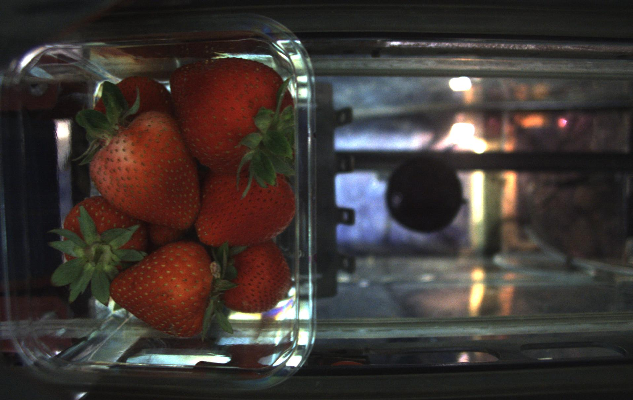
\includegraphics[width=.9\linewidth]{bg_example.png}
		\caption{}
		\label{fig:bg_example}
	\end{subfigure}%
	\begin{subfigure}{.4\textwidth}
		\centering
		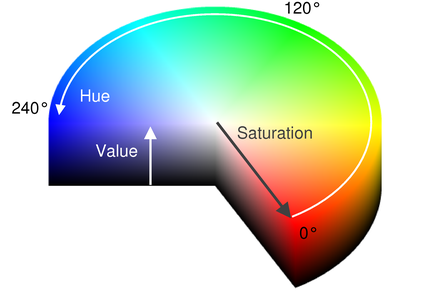
\includegraphics[width=.9\linewidth]{hue_sat.png}
		\caption{}
		\label{fig:hue_sat}
	\end{subfigure}%

	\begin{subfigure}{.4\textwidth}
		\centering
		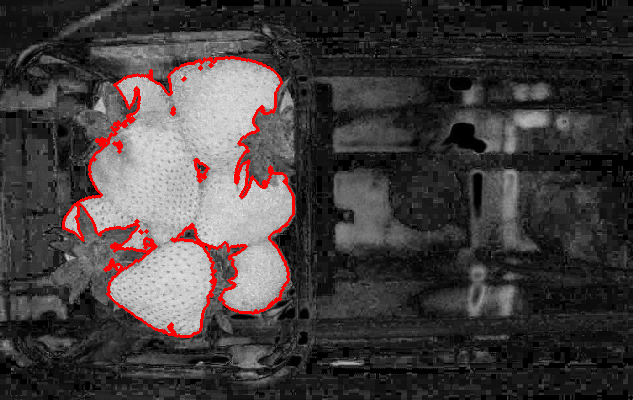
\includegraphics[width=.9\linewidth]{sat_thresh.png}
		\caption{}
		\label{fig:sat_thresh}
	\end{subfigure}%
	\begin{subfigure}{.4\textwidth}
		\centering
		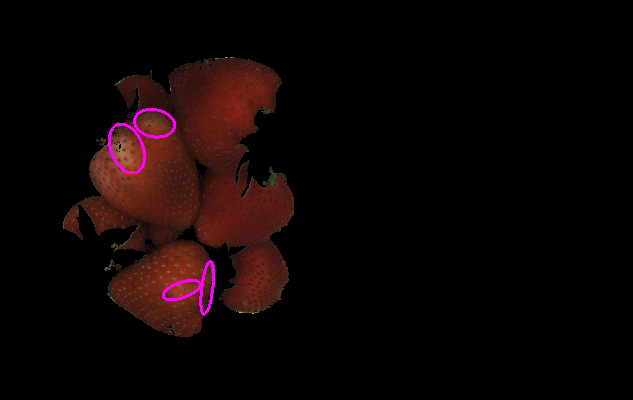
\includegraphics[width=.9\linewidth]{hue_processed.png}
		\caption{}
		\label{fig:hue_processed}
	\end{subfigure}%

	\caption{Left to right: (a)Example of background noise with white light and bottom camera lens in background, (b)HSV colourspace showing hue circle and saturation vector, (c)Saturation channel with berries segmented after pre-processing, (d)Image reduced to berry region showing four small under ripe areas detected by the algorithm.}
	\label{fig:test2}
\end{figure}



\subsection{Implementation and Results}

The enclosure was firstly constructed offline as a bench prototype (Fig. \ref{fig:bench_construct}), in order to test lighting arrangements, polarizers, and cameras. This prototype was then used as the framework when moved from bench to production. 

Several lighting and polarizing configurations were tested for optimization (Figures \ref{fig:bench_hal_film} and \ref{fig:bench_hal_film2}). Before the AC flickering problem was realised, halogen work lamps were tested as the main lighting source, with a thin film type polaroid. This test was successful in prooving that the polarizer reduced specularities, and that powerful lighting was required, however, it highlighted the inherant problem with AC lighting and fast shutter speeds. It was also noted during these preliminary tests that the polarizer film would be less effective when bent or warped.  

Converting the system to $12V$ power was required in order to provide a more constant current and, therefore, lighting intensity. Auotomotive LED light bars replaced the halogen work lamps for the visible spectrum, whilst $12V/35W$ halogen down lights provide the IR spectrum as shown in figures \ref{fig:bench_led_rigid} and \ref{fig:production_LED_Hal}. 

\begin{wrapfigure}{r}{0.5\textwidth}
	\begin{center}
		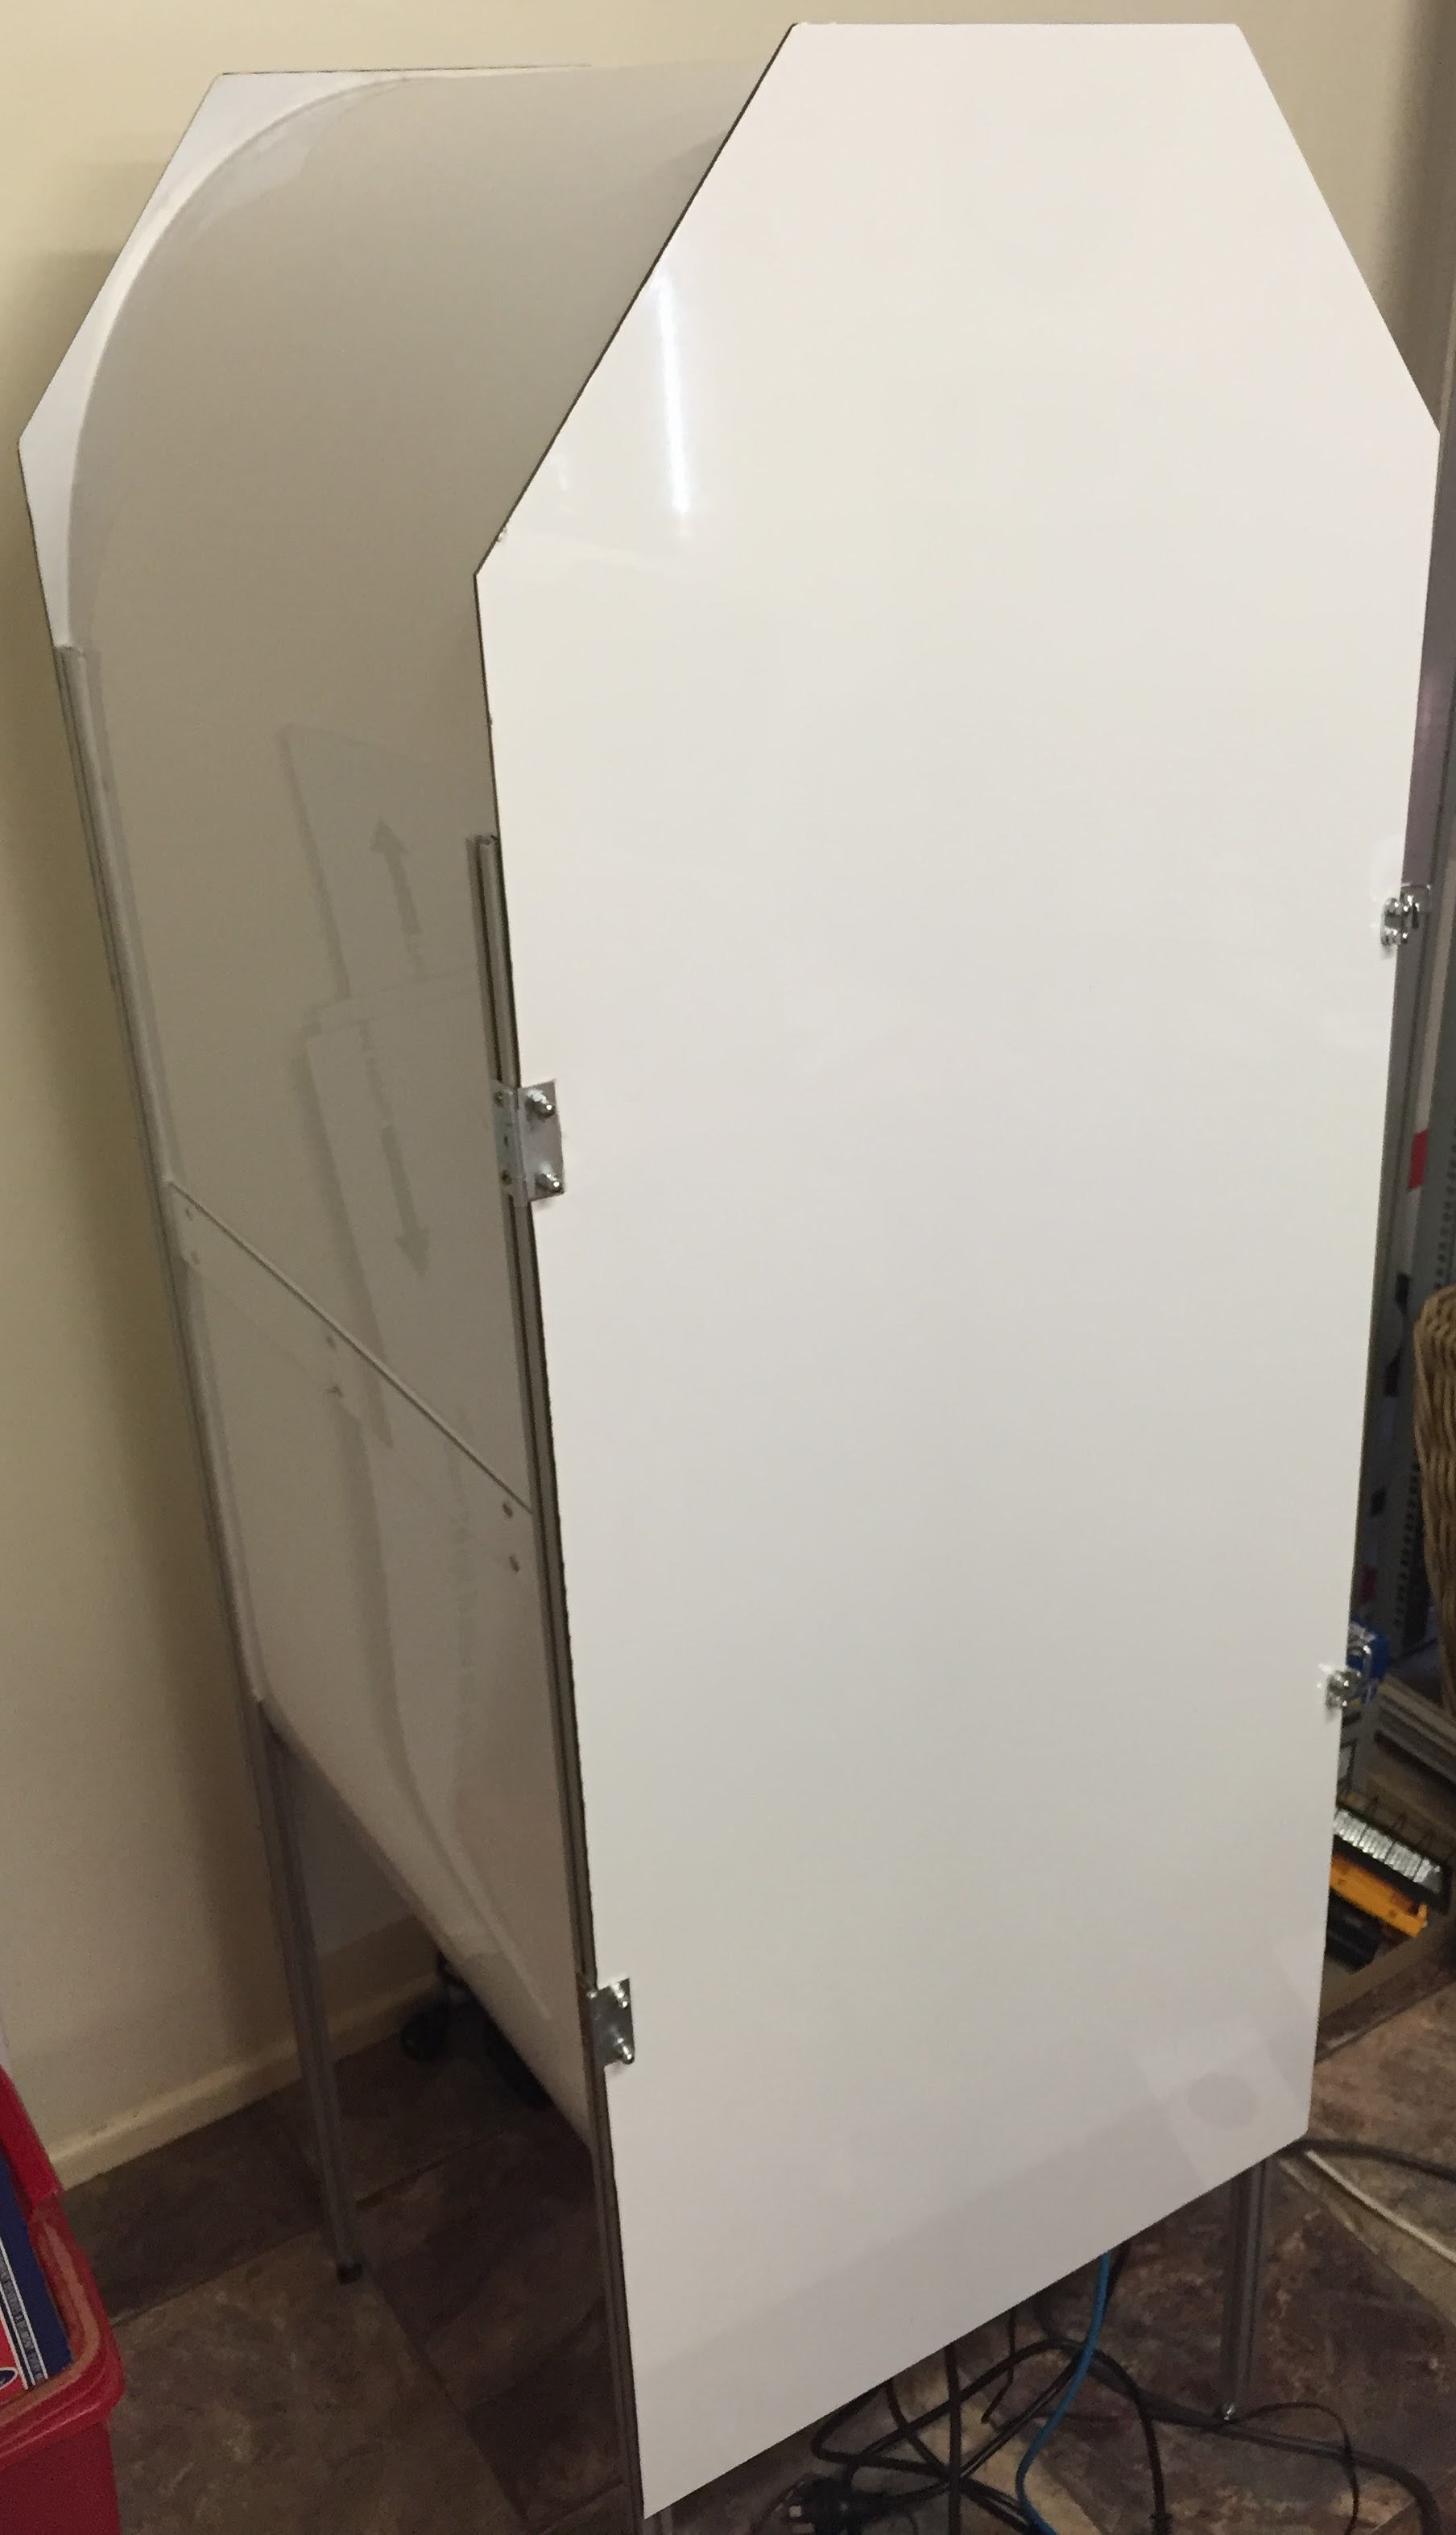
\includegraphics[width=0.3\textwidth]{images/bench_construct.jpg}
	\end{center}
	\caption{The enclosed prototype during construction and testing.}
	\label{fig:bench_construct}
\end{wrapfigure}   

The final production version is an in-line system with a conveyor feeding into and out of the camera enclosure. Therefore, the external cladding was modified to allow the conveyors entry and exit points without allowing external, potentially noisy, light leaking inside. This was ensured by constructing a protruding tunnel on both sides of the enclosure as shown in the final setup in figure \ref{fig:production_final}.

A touchscreen was also installed to allow operators and developers easy access to the UI buttons and display. The commercially available Dell \textcopyright P2418HT 24-inch capacitive touch screen can help development as well as production with the ability to debug whilst on the production line.


\begin{figure}[h]
	\centering
	\begin{subfigure}{.35\textwidth}
		\centering
		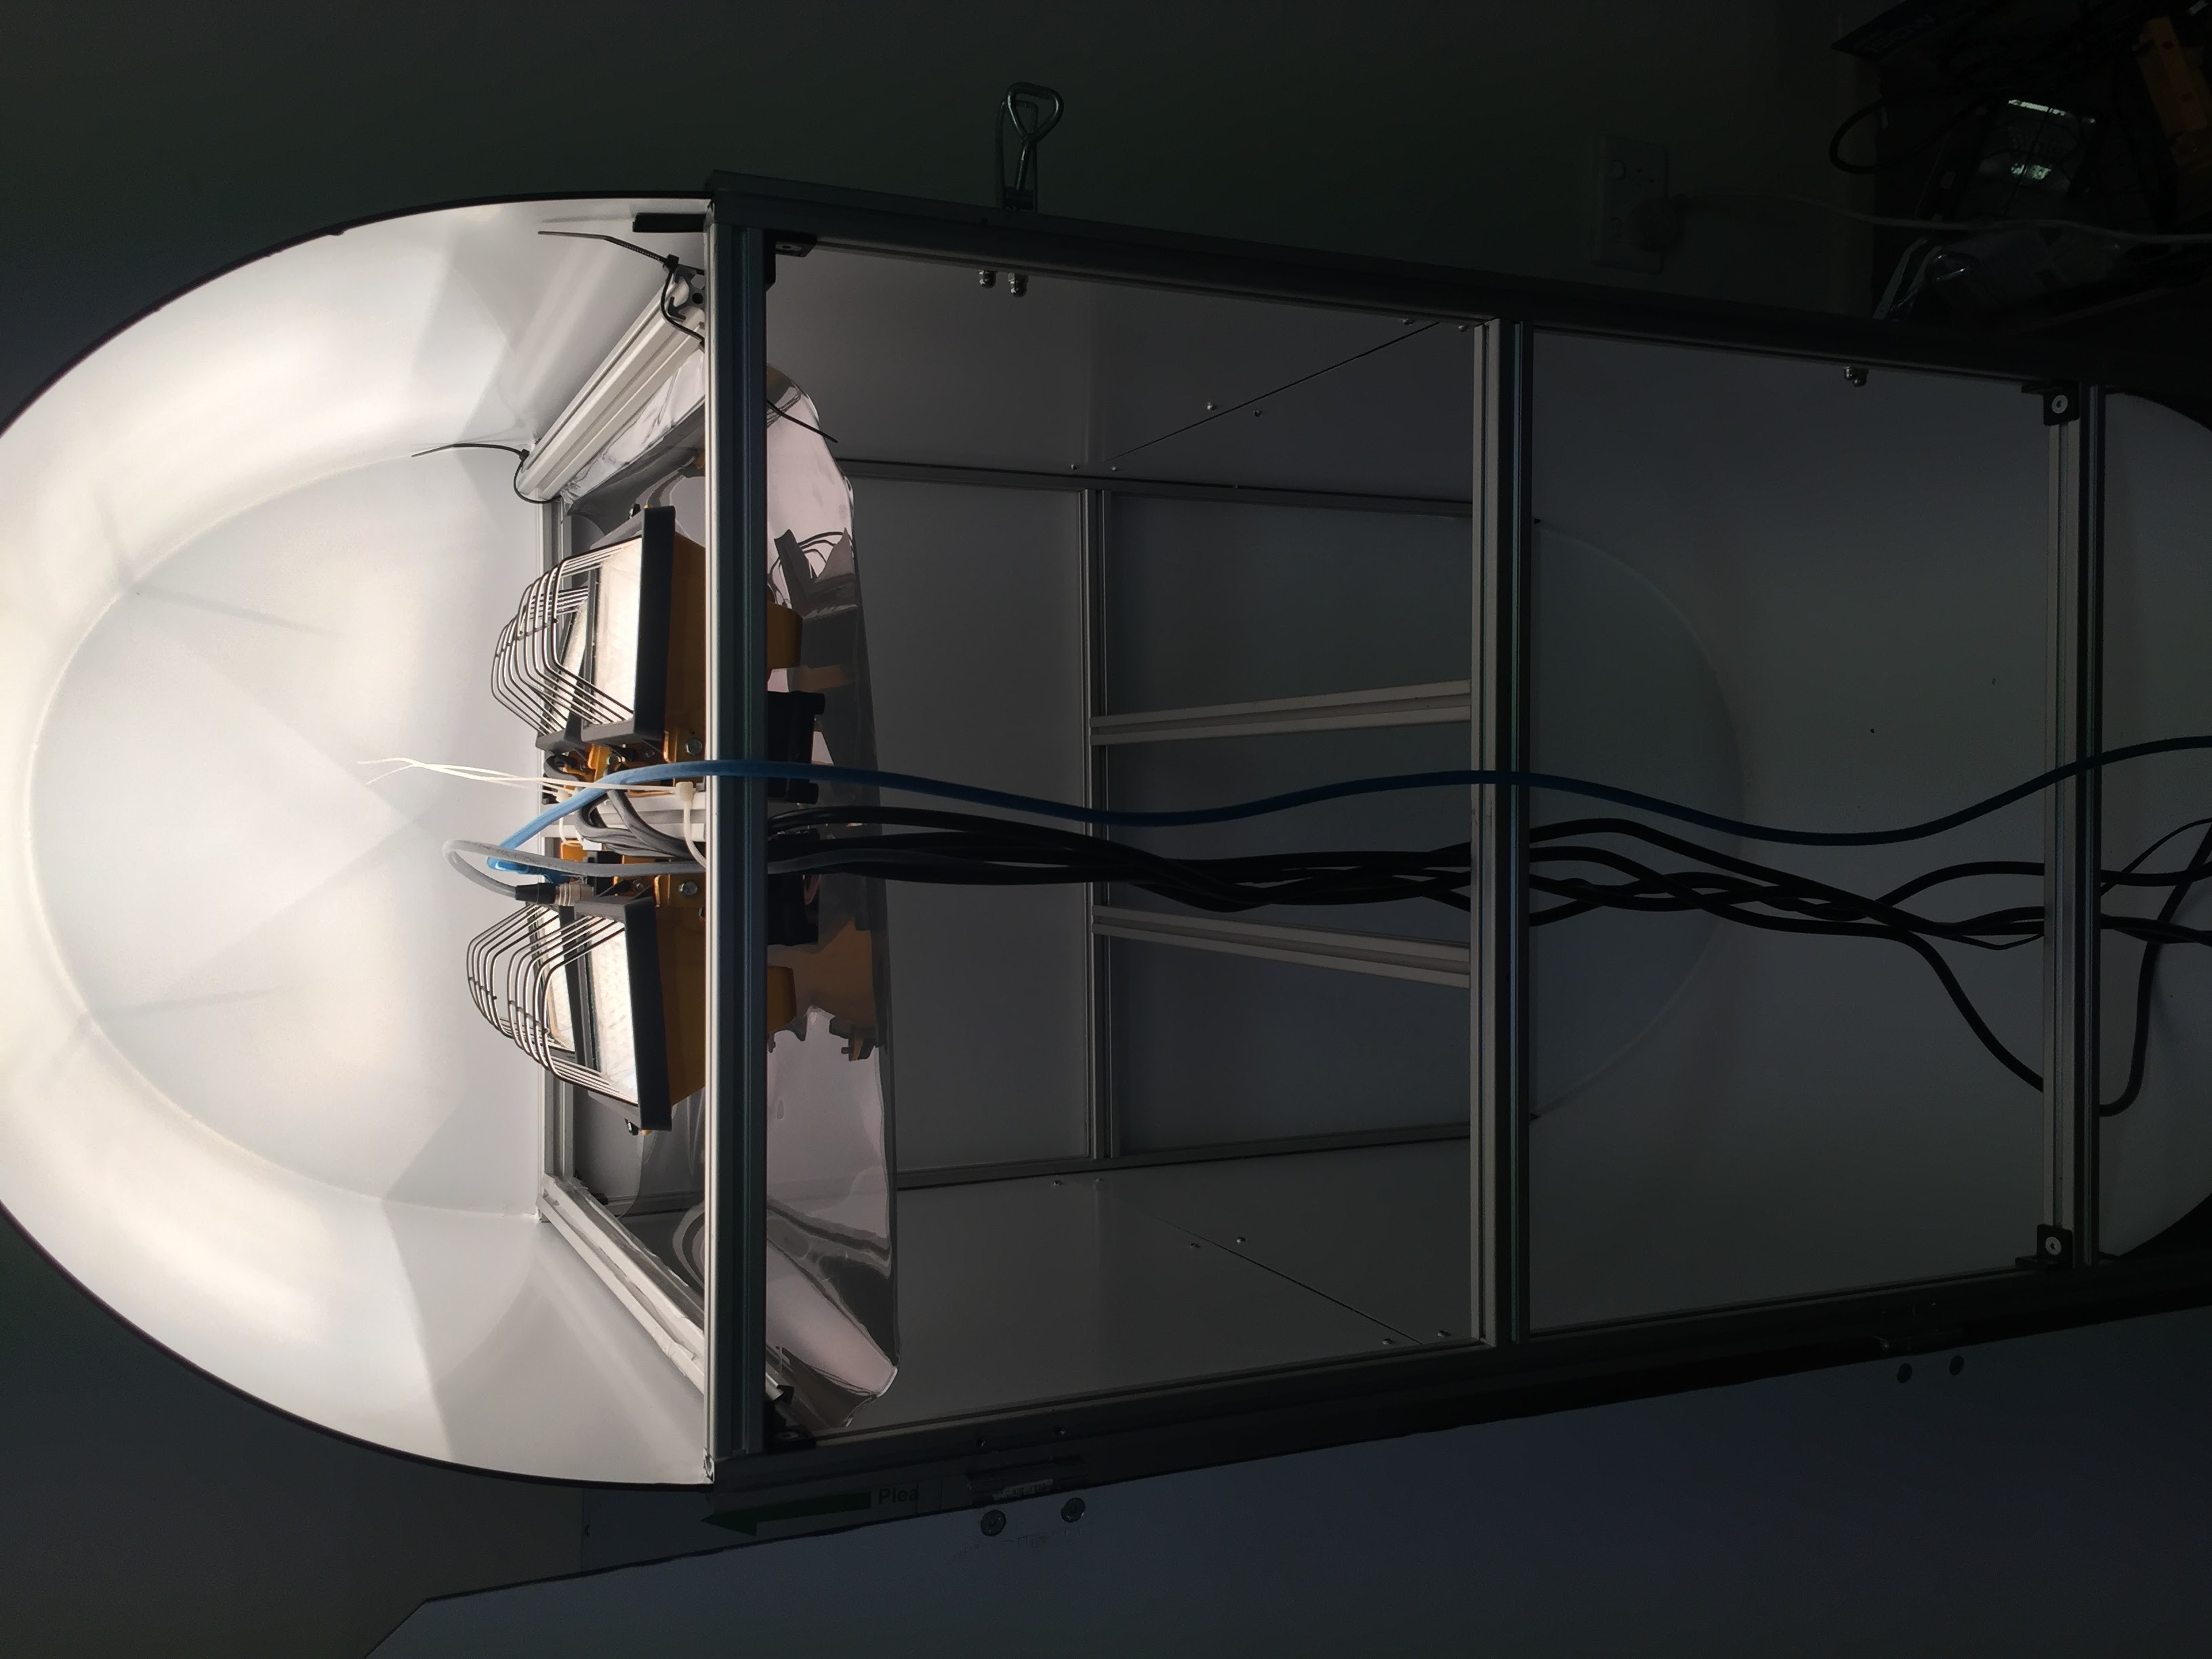
\includegraphics[width=.9\linewidth,angle=270,origin=c]{bench_hal_film.jpg}
		\caption{}
		\label{fig:bench_hal_film}
	\end{subfigure}%
	\begin{subfigure}{.35\textwidth}
		\centering
		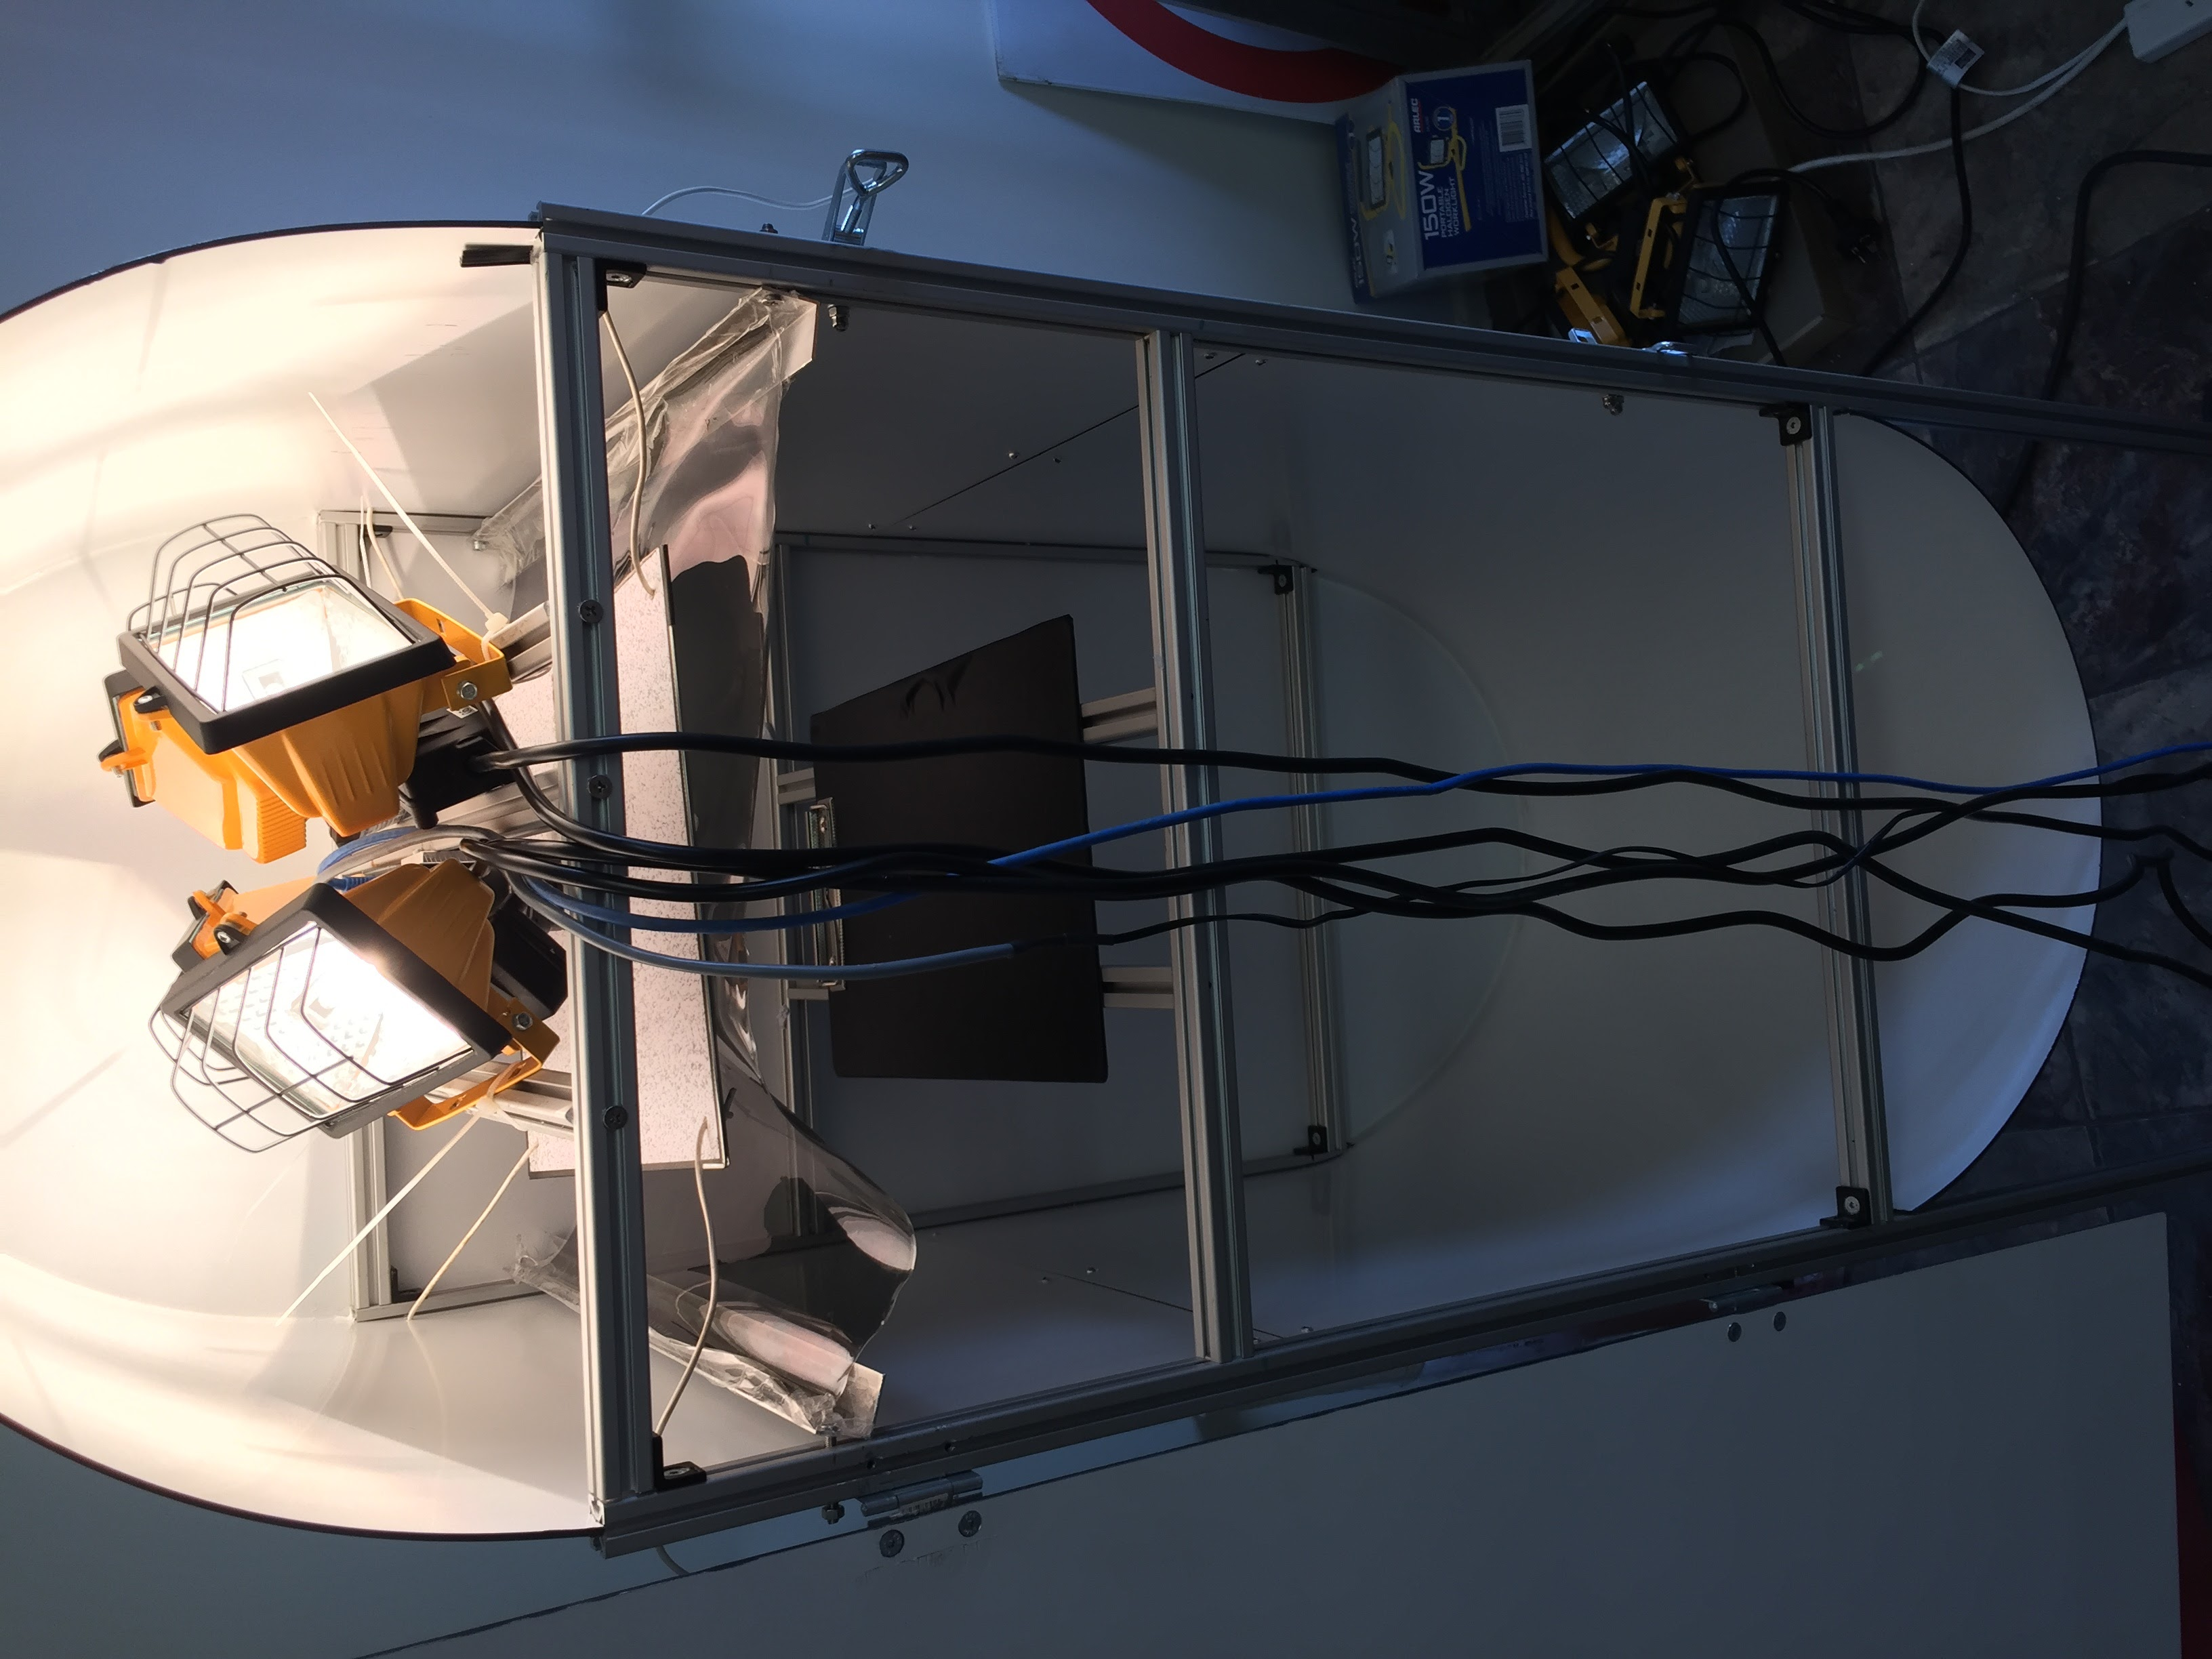
\includegraphics[width=.9\linewidth,angle=270,origin=c]{bench_hal_film2.jpg}
		\caption{}
		\label{fig:bench_hal_film2}
	\end{subfigure}%
	
	\begin{subfigure}{.35\textwidth}
		\centering
		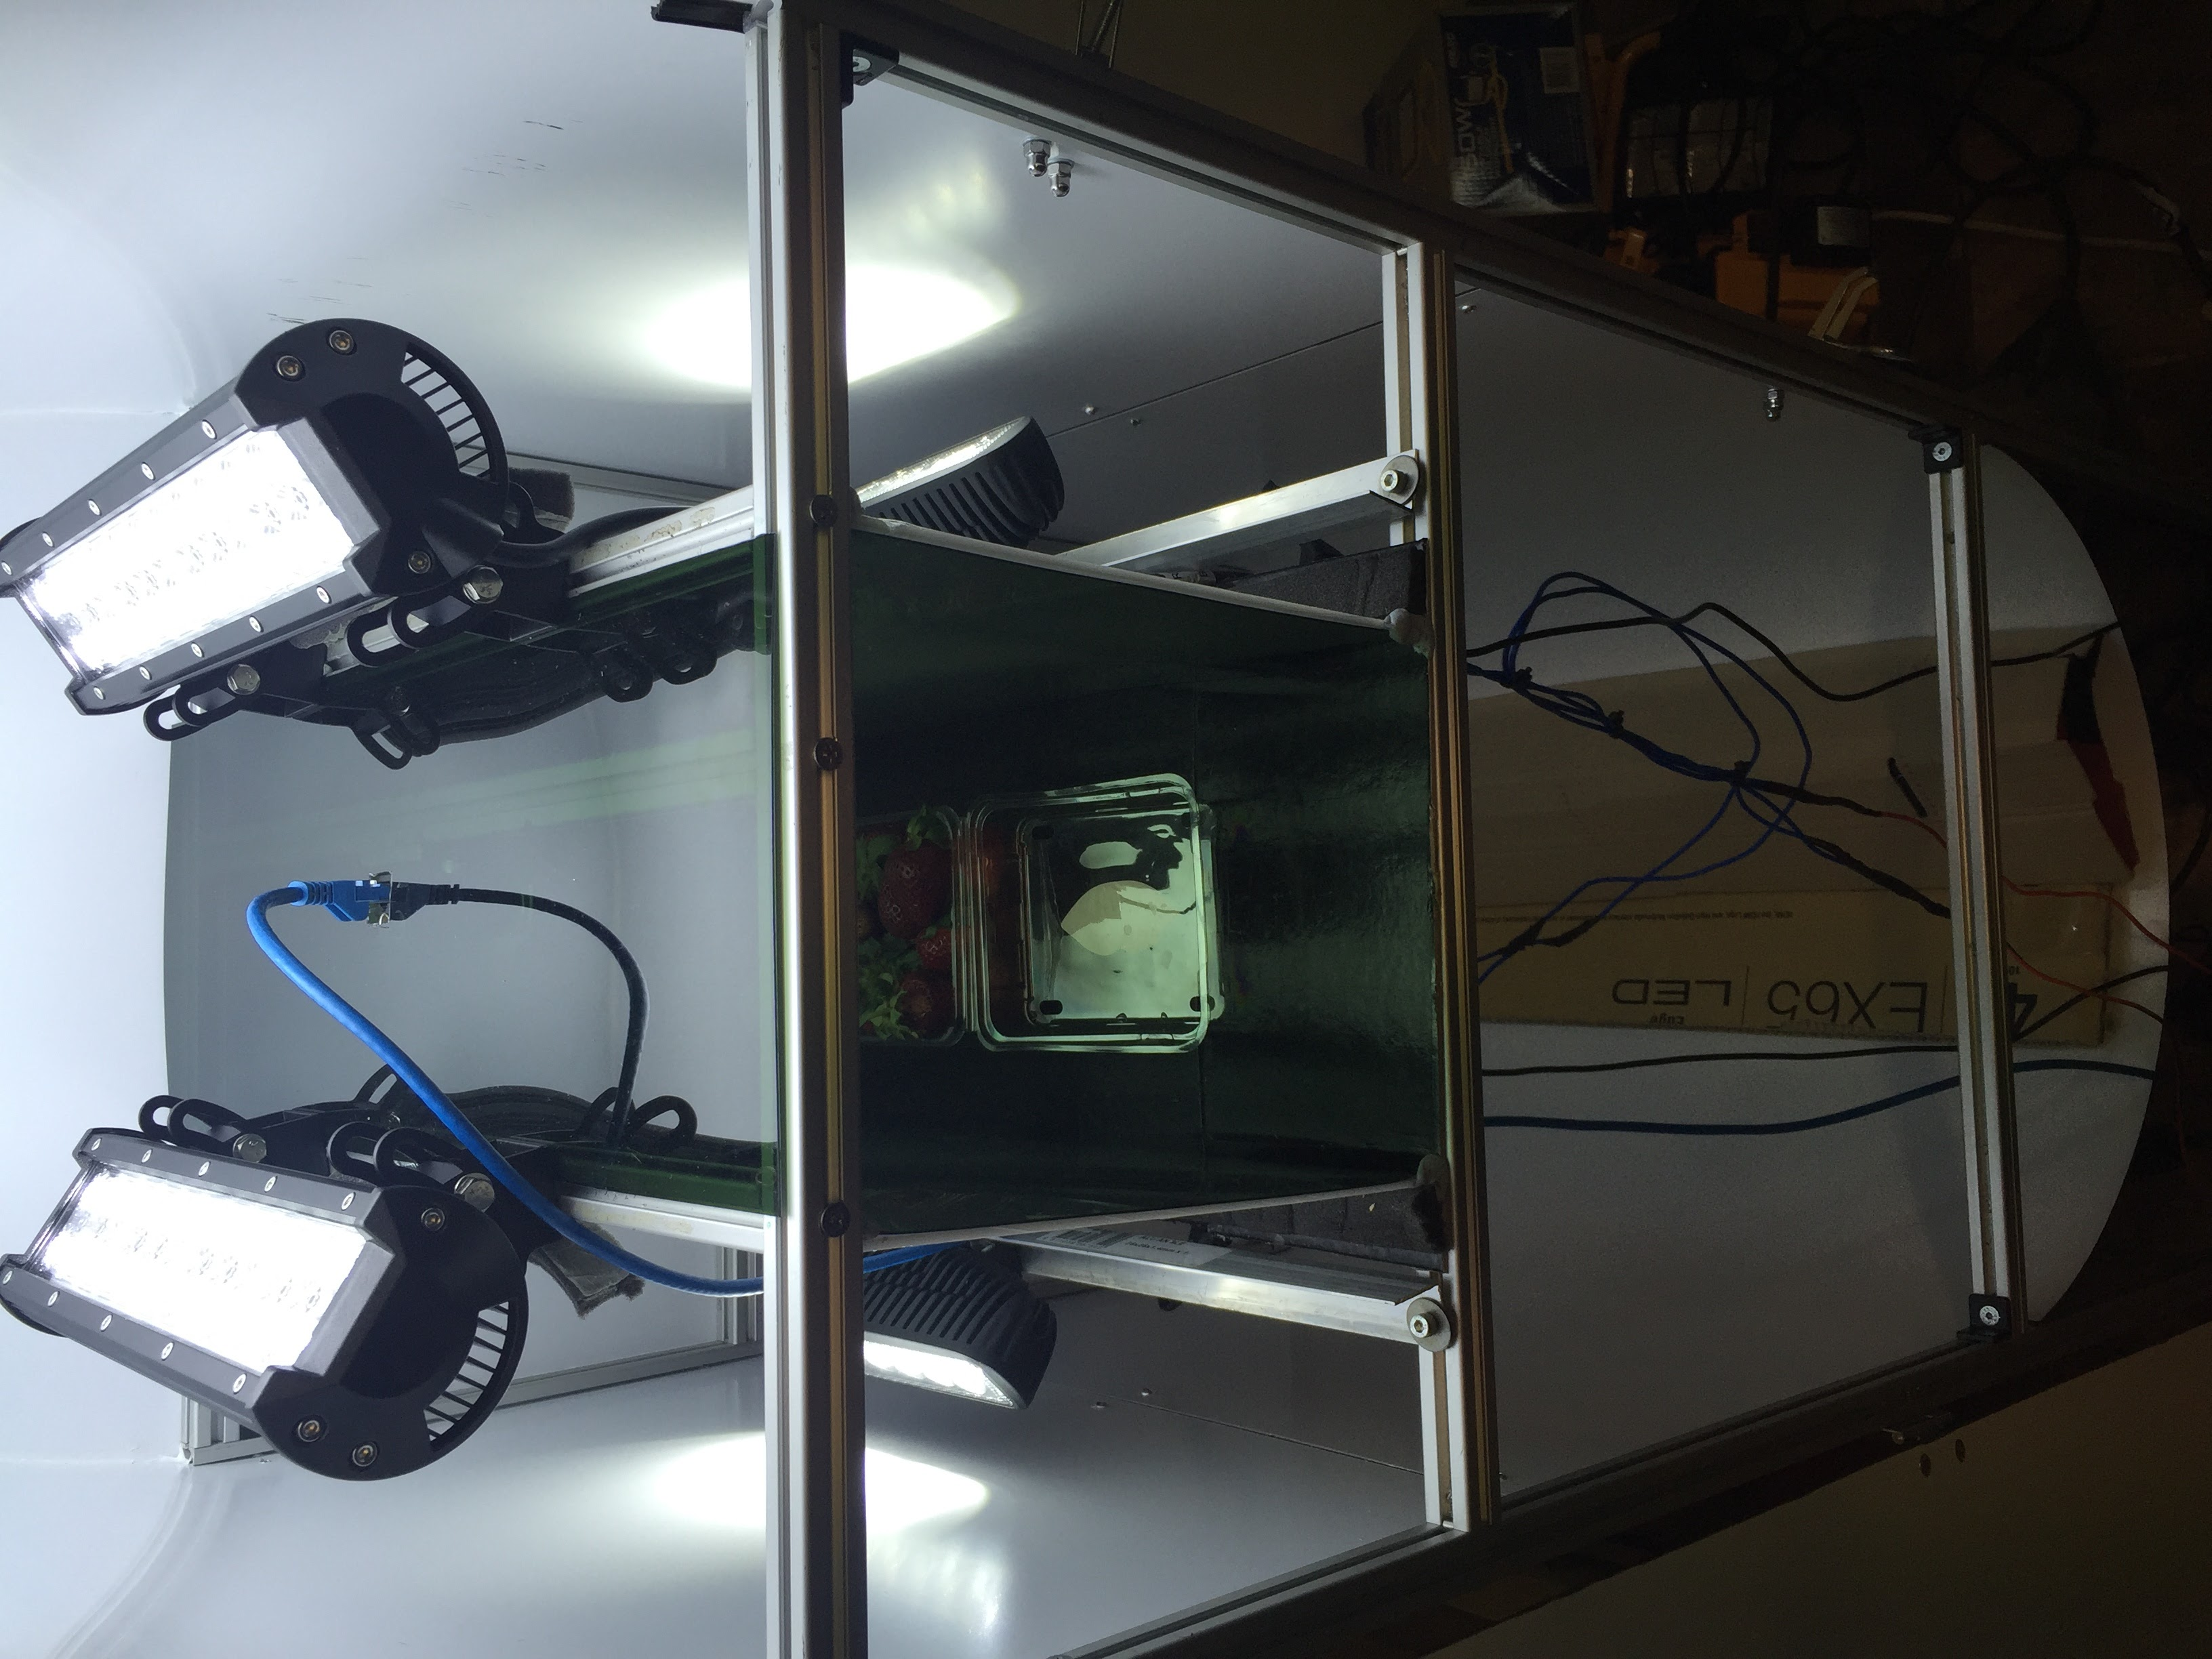
\includegraphics[width=.9\linewidth,angle=270,origin=c]{bench_led_rigid.jpg}
		\caption{}
		\label{fig:bench_led_rigid}
	\end{subfigure}%
	\begin{subfigure}{.35\textwidth}
		\centering
		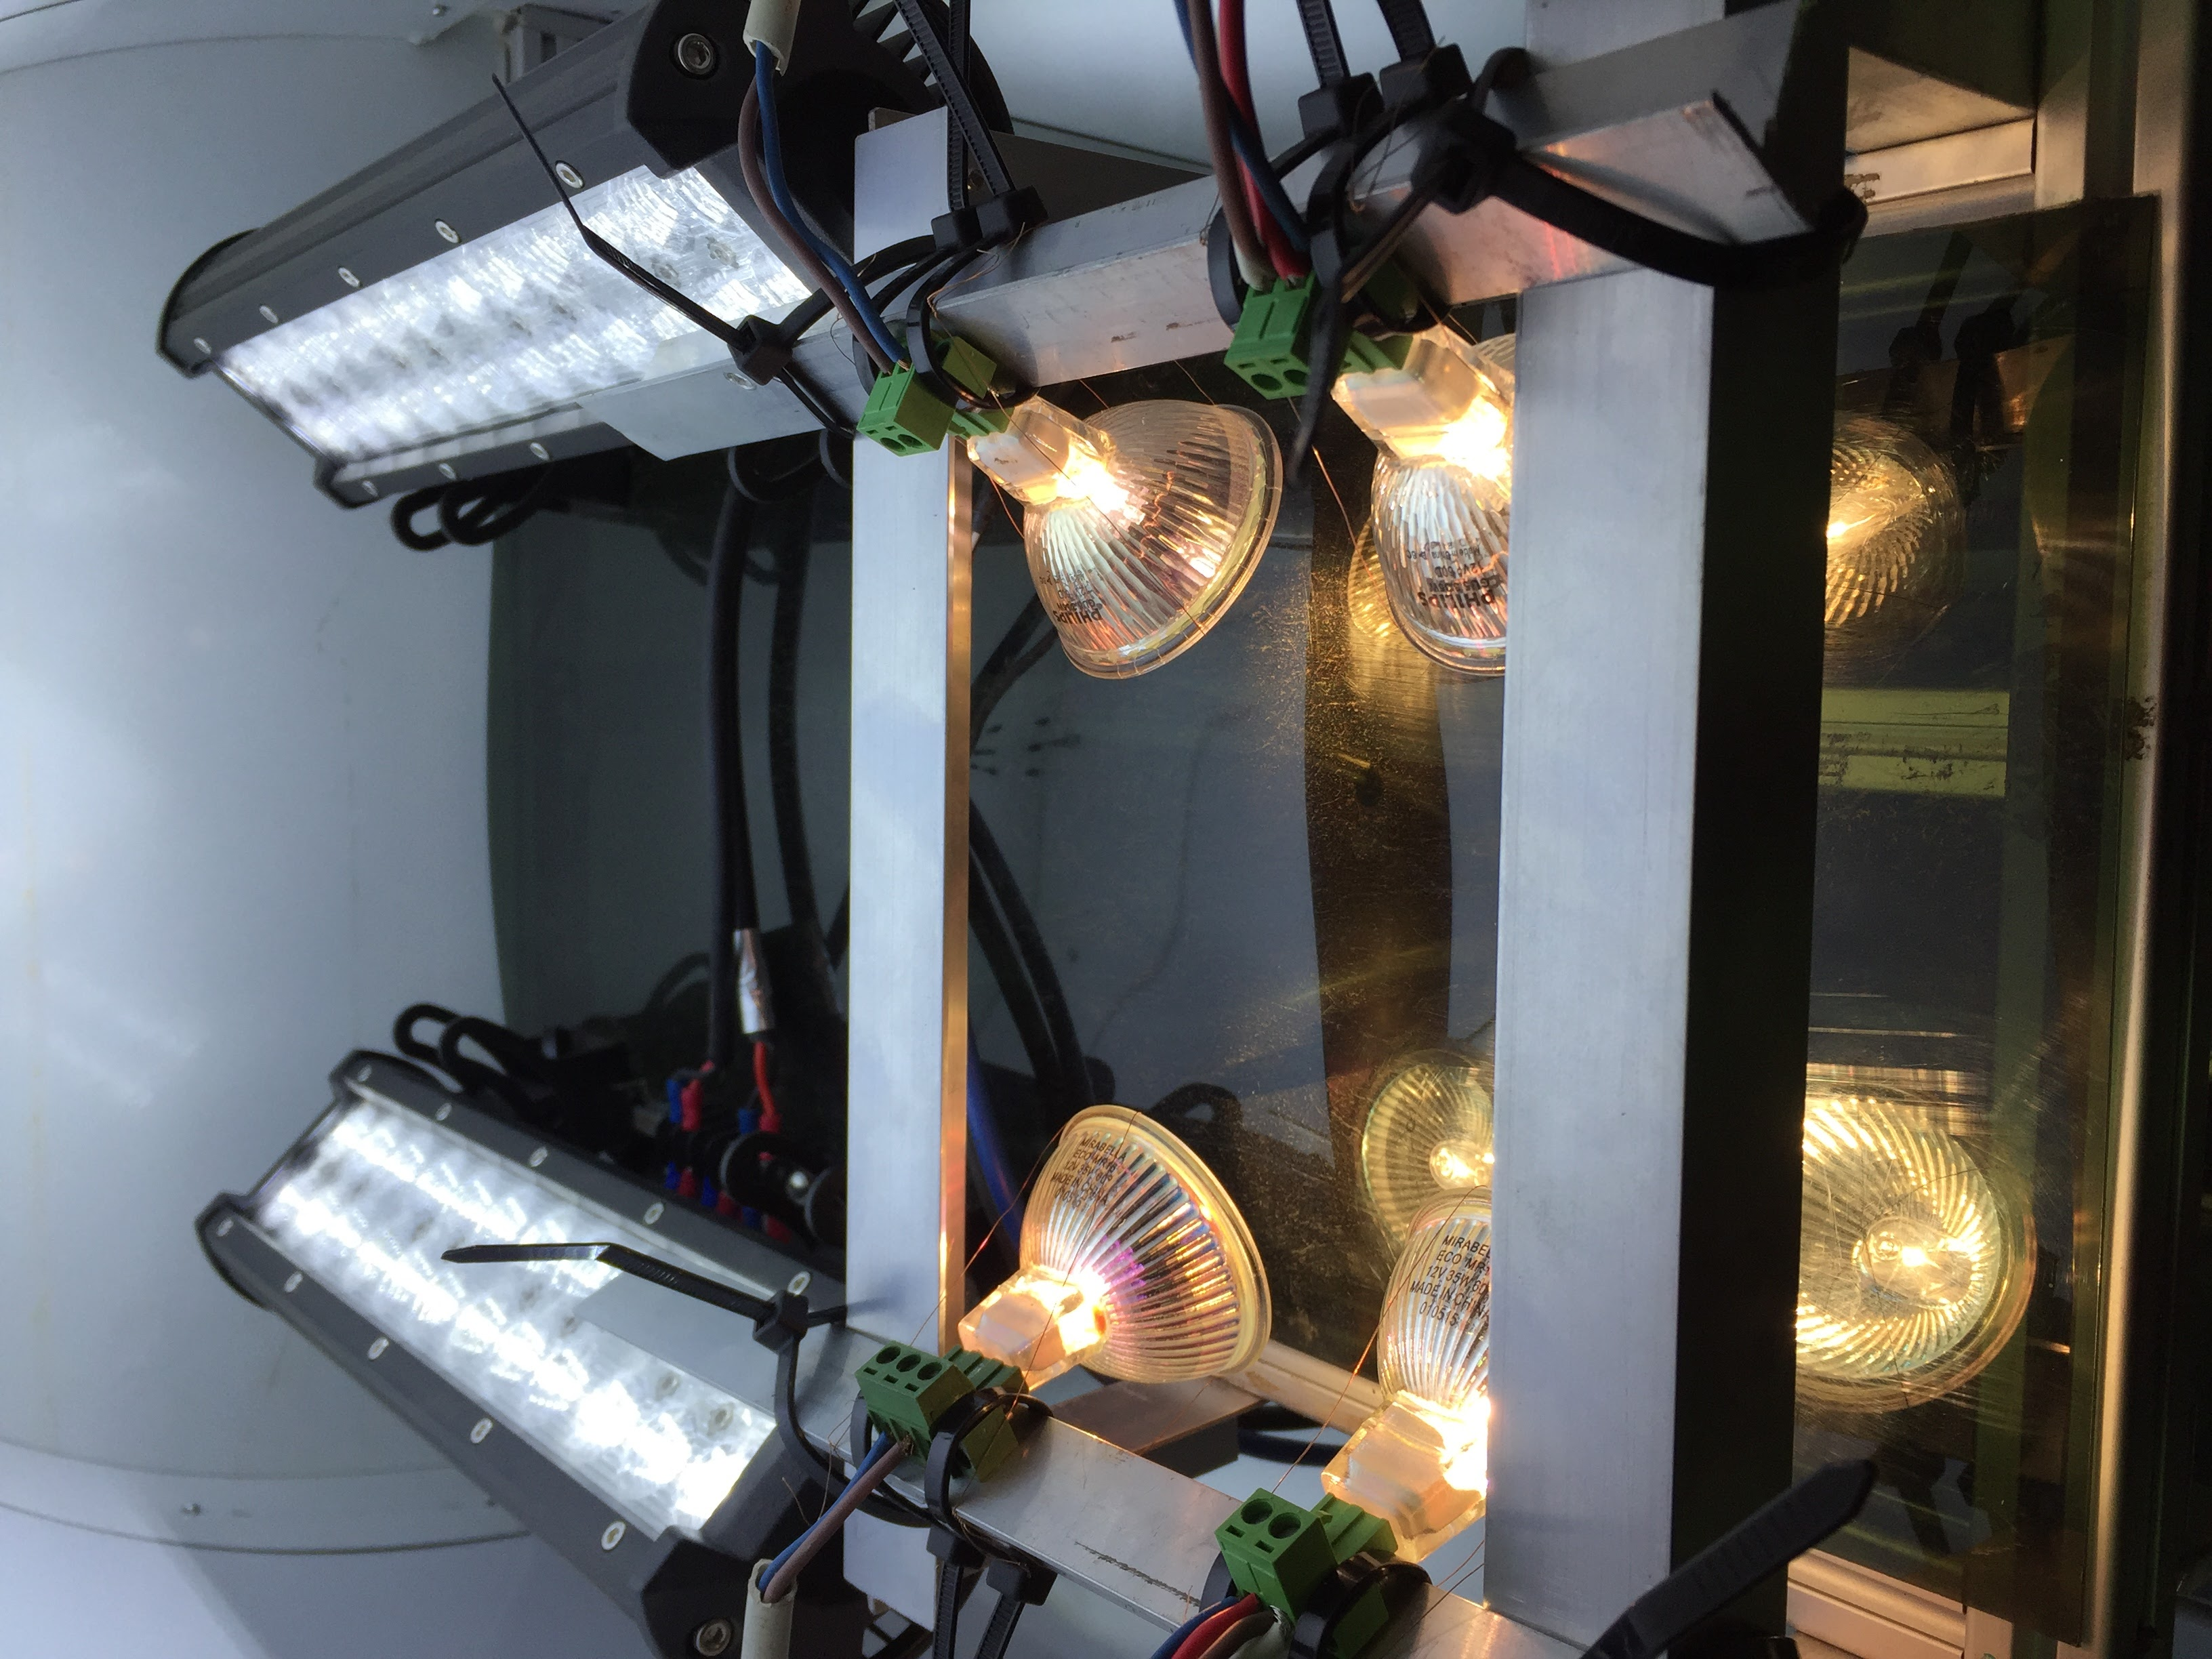
\includegraphics[width=.9\linewidth,angle=270,origin=c]{images/production_LED_Hal.jpg}
		\caption{}
		\label{fig:production_LED_Hal}
	\end{subfigure}%
	
	\caption{Left to right: (a)Halogen work lamps tested facing upwards with a thin film polaroid , (b)Halogen work lamps in a diagolally upward direction with a dark-field blocker, (c)Installation of LED light bars and rigid polarizing material, (d)Installation of $12V$ halogen down lights.}
	\label{fig:test3}
\end{figure}


The ejector system was installed at a later date as further testing was required to ensure the proper ejection of the punnets. The ejector had to be calibrated to give the correct amount of force to remove the punnet gently but definately. The punnet identified as poor quality must also be ejected at a later stage (after the punnet leaves the enclosure), therefore the ejector must synchronise with the punnet detector/cameras.

Operators have given good feedback and that the ejected punnets were confirmed as under ripe. A start up procedure has been documented and is in use so that the operators can start and stop the vision system when required and therefore will not require constant monitoring by the developers. Since installation on the production line, a dataset of $>30,000$ punnets has been acquired, with 2-4 images per punnet from each orientaion and wavelength. The system has ejected 67 punnets since the ejector was turned on - just over one month of production - keeping in mind that the only algorithm implemented at this time was the under ripe detection. The ejector was turned on towards the end of the season, which meant that the fruit had had many months to ripen. Recently, two more algorithms were added to the repertoir and are in the confirmation stage at present, with the addition of several more to come in the near future.


\begin{figure}[ht]
	\centering
	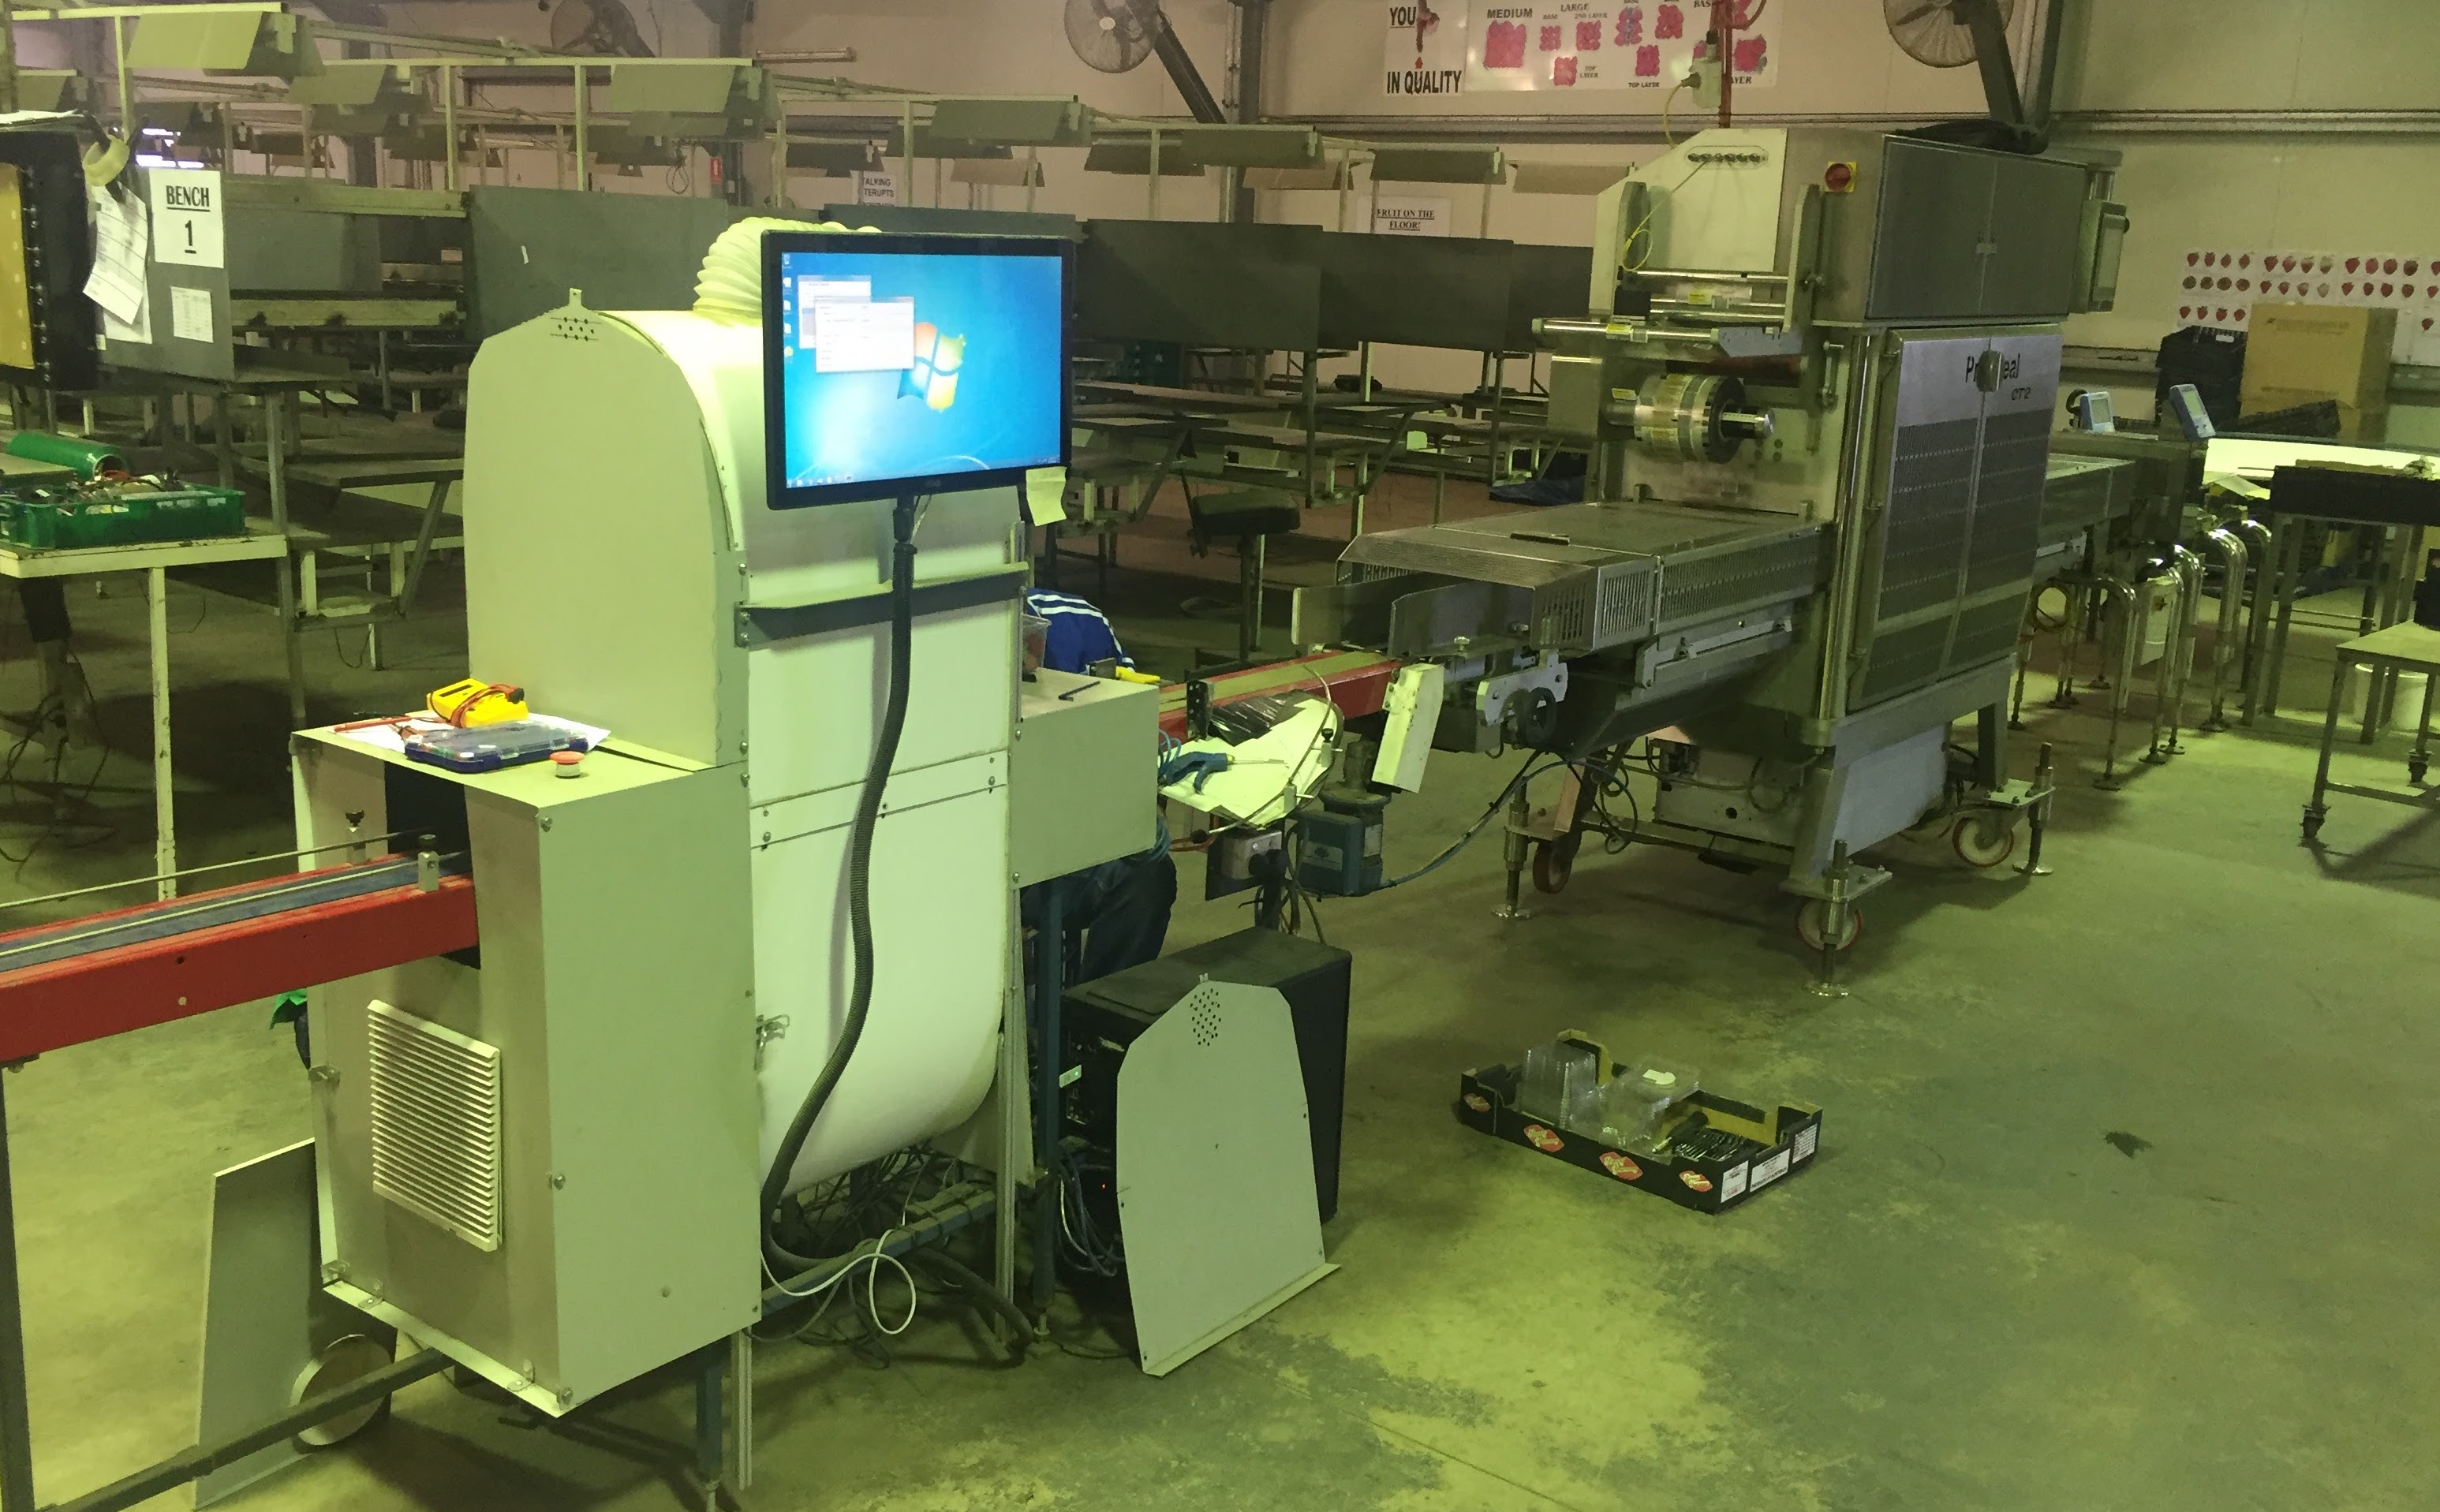
\includegraphics[width=0.8\textwidth]{images/production_final.JPG}
	\caption{SQA enclosure with touchscreen and cladding. The SQA system feeds into the heat seal machine directly.}
	\label{fig:production_final}
\end{figure}


A dataset of 500+ images has been truthed by operators and used to assess the algorithms implemented. The current under ripe algorithm had very good results at $89.11\%$ accuracy. Examples of typical under ripe rejections is shown in Figure \ref{fig:UR_berries}.


\begin{figure}[h]
	\centering
	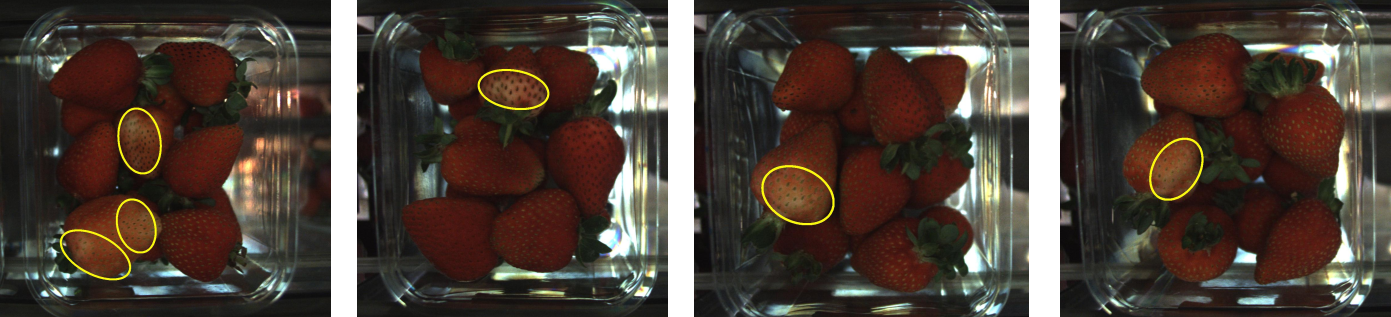
\includegraphics[width=0.9\textwidth]{UR_berries.png}
	\caption{Examples of under ripe berry detection in full punnets.}
	\label{fig:UR_berries}
\end{figure}


%%%%%%%%%%%%%%%%%%%%%%%%%%%%%%%%%%%%%%%%%%%%%%%%%%%%%%%%%%%%%%%%%%%%%%%%%%%%%%
%%%%%%%%%%%%%%%%%%%%%%%%%%%%%%%%%%%%%%%%%%%%%%%%%%%%%%%%%%%%%%%%%%%%%%%%%%%%%%


\section{II - Production Integration}











%%%%%%%%%%%%%%%%%%%%%%%%%%%%%%%%%%%%%%%%%%%%%%%%%%%%%%%%%%%%%%%%%%%%%%%%%%%%%%
%%%%%%%%%%%%%%%%%%%%%%%%%%%%%%%%%%%%%%%%%%%%%%%%%%%%%%%%%%%%%%%%%%%%%%%%%%%%%%


\section{III - System Reconfiguration and Redesign}















%%%%%%%%%%%%%%%%%%%%%%%%%%%%%%%%%%%%%%%%%%%%%%%%%%%%%%%%%%%%%%%%%%%%%%%%%%%%%%
%%%%%%%%%%%%%%%%%%%%%%%%%%%%%%%%%%%%%%%%%%%%%%%%%%%%%%%%%%%%%%%%%%%%%%%%%%%%%%


\section{IV - Linux and Deep Learning}















%%%%%%%%%%%%%%%%%%%%%%%%%%%%%%%%%%%%%%%%%%%%%%%%%%%%%%%%%%%%%%%%%%%%%%%
%%%%%%%%%%%%%%%%%%%%%%%%%%%%%%%%%%%%%%%%%%%%%%%%%%%%%%%%%%%%%%%%%%%%%%%


\section{Conclusion}














%%%%%%%%%%%%%%%%%%%%%%%%%%%%%%%%%%%%%%%%%%%%%%%%%%%%%%%%%%%%%%%%%%%%%%%
%%%%%%%%%%%%%%%%%%%%%%%%%%%%%%%%%%%%%%%%%%%%%%%%%%%%%%%%%%%%%%%%%%%%%%%


\newpage
\bibliographystyle{ieeetr}
\bibliography{Master}



%%%%%%%%%%%%%%%%%%%%%%%%%%%%%%%%%%%%%%%%%%%%%%%%%%%%%%%%%%%%%%%%%%%%%%%%
%%%%%%%%%%%%%%%%%%%%%%%%%%%%%%%%%%%%%%%%%%%%%%%%%%%%%%%%%%%%%%%%%%%%%%%%


% that's all folks
\end{document}